\documentclass[11pt]{book}

\usepackage[margin=1in]{geometry}
\usepackage{amsmath,amssymb,amsthm,mathtools}
\usepackage{array}
\usepackage{enumitem}
\usepackage{hyperref}
\usepackage{tikz}
\usetikzlibrary{arrows.meta,calc,positioning,decorations.markings,
  decorations.pathmorphing,patterns,shadings,shapes.geometric,fadings,
  backgrounds,intersections,bending}
\usepackage{thmtools}
\usepackage{cleveref}

% Monochrome palette for classic textbook-style figures.  The imported TikZ
% figures use these semantic color names; mapping them to black/gray removes
% color while preserving line weights, fills, and diagram structure.
\definecolor{formteal}{gray}{0.00}
\definecolor{formgold}{gray}{0.00}
\definecolor{formrust}{gray}{0.00}
\definecolor{formplum}{gray}{0.00}
\definecolor{formsage}{gray}{0.00}
\definecolor{formslate}{gray}{0.00}
\definecolor{formivory}{gray}{1.00}

\newcommand{\sagedir}{../sagemath}
\input{\sagedir/coords.tex}
\input{\sagedir/coords_torus.tex}
\input{\sagedir/coords_curve_sample.tex}

\newcommand{\drawprecisetorus}{%
  \fill[formteal!13, line join=round] plot[smooth cycle] coordinates {\torusOuter};
  \fill[white, line join=round] plot[smooth cycle] coordinates {\torusInner};
  \foreach \name in {Zero,One,Two,Three,Four,Five,Six,Seven}{%
    \draw[draw=formteal!60!black, line width=0.42pt, line join=round, opacity=0.9]
      plot[smooth] coordinates {\csname torusMer\name VA\endcsname};}
  \draw[draw=formteal!60!black, line width=0.42pt, line join=round, opacity=0.9]
    plot[smooth] coordinates {\torusMerFiveVB};
  \draw[draw=formteal!60!black, line width=0.42pt, line join=round, opacity=0.9]
    plot[smooth] coordinates {\torusMerSixVB};
  \draw[draw=formteal!60!black, line width=0.42pt, line join=round, opacity=0.9]
    plot[smooth] coordinates {\torusMerSevenVB};
  \draw[draw=formteal!60!black, line width=0.5pt, line join=round, opacity=0.95]
    plot[smooth] coordinates {\torusLonTopVA};
  \draw[draw=formteal!60!black, line width=0.42pt, line join=round, opacity=0.8]
    plot[smooth] coordinates {\torusLonOuterVA};
  \draw[draw=formteal!60!black, line width=0.42pt, line join=round, opacity=0.8]
    plot[smooth] coordinates {\torusLonInnerVA};
  \draw[draw=formteal!65!black, line width=0.95pt, line join=round]
    plot[smooth cycle] coordinates {\torusOuter};
  \draw[draw=formteal!65!black, line width=0.8pt, line join=round]
    plot[smooth cycle] coordinates {\torusInner};
}

\newcommand{\drawprecisecurve}{%
  \draw[draw=formteal!60!black, line width=0.88pt, line join=round]
    plot[smooth cycle, tension=0.85] coordinates {\curveOvalFull};
  \draw[draw=formteal!60!black, line width=0.88pt, line join=round]
    plot[smooth, tension=0.9] coordinates {\curveBranchUpper};
  \draw[draw=formteal!60!black, line width=0.88pt, line join=round]
    plot[smooth, tension=0.9] coordinates {\curveBranchLower};
  \fill[formteal!70!black] (-1,0) circle (1.8pt);
  \fill[formteal!70!black] ( 0,0) circle (1.8pt);
  \fill[formteal!70!black] ( 1,0) circle (1.8pt);
}

\newcommand{\classicTrinityDiagram}{%
  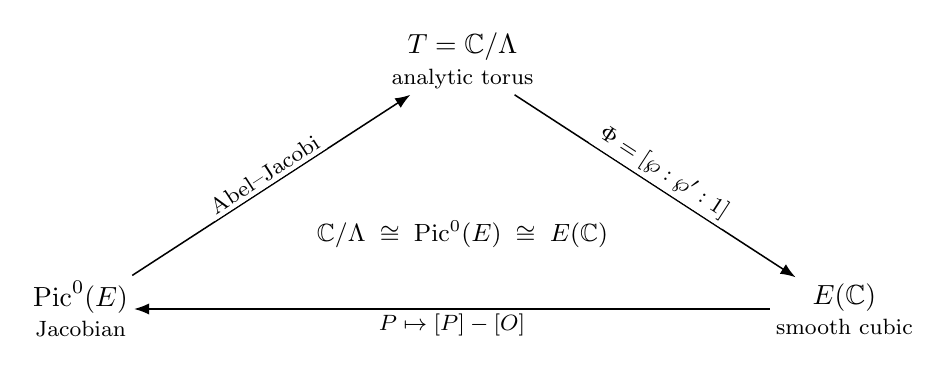
\begin{tikzpicture}[>=Latex,
      object/.style={align=center, inner sep=2pt},
      map/.style={->, line width=0.55pt},
      lab/.style={font=\footnotesize, fill=white, inner sep=1.5pt}]
    \node[object] (T) at (0,3.15)
      {$T=\C/\Lambda$\\[-1pt]{\footnotesize analytic torus}};
    \node[object] (E) at (4.85,0)
      {$E(\C)$\\[-1pt]{\footnotesize smooth cubic}};
    \node[object] (J) at (-4.85,0)
      {$\Pic^0(E)$\\[-1pt]{\footnotesize Jacobian}};
    \draw[map] (T) -- node[lab, sloped, above] {$\Phi=[\wp:\wp':1]$} (E);
    \draw[map] (E) -- node[lab, below] {$P\mapsto [P]-[O]$} (J);
    \draw[map] (J) -- node[lab, sloped, above] {Abel--Jacobi} (T);
    \node[font=\small] at (0,0.95)
      {$\C/\Lambda\;\cong\;\Pic^0(E)\;\cong\;E(\C)$};
  \end{tikzpicture}%
}

\newcommand{\classicChordDiagram}{%
  \begin{tikzpicture}[scale=1.0, every node/.style={font=\small}]
    \draw[->, black!55, line width=0.45pt] (-1.7,0) -- (2.7,0) node[right] {$x$};
    \draw[->, black!55, line width=0.45pt] (0,-3.3) -- (0,3.5) node[above] {$y$};
    \drawprecisecurve
    \draw[black, line width=0.65pt]
      (\chordlefta,\chordleftb) -- (\chordrighta,\chordrightb);
    \draw[dashed, black!65, line width=0.45pt]
      (\chordRx,\chordRy) -- (\chordSx,\chordSy);
    \fill[black] (\chordPx,\chordPy) circle (2.1pt);
    \node[above left] at (\chordPx,\chordPy) {$P$};
    \fill[black] (\chordQx,\chordQy) circle (2.1pt);
    \node[above right] at (\chordQx,\chordQy) {$Q$};
    \fill[black] (\chordRx,\chordRy) circle (2.1pt);
    \node[above left] at (\chordRx,\chordRy) {$R$};
    \fill[black] (\chordSx,\chordSy) circle (2.3pt);
    \node[below left] at (\chordSx,\chordSy) {$P\oplus Q=-R$};
  \end{tikzpicture}%
}

\newcommand{\classicExpSequenceDiagram}{%
  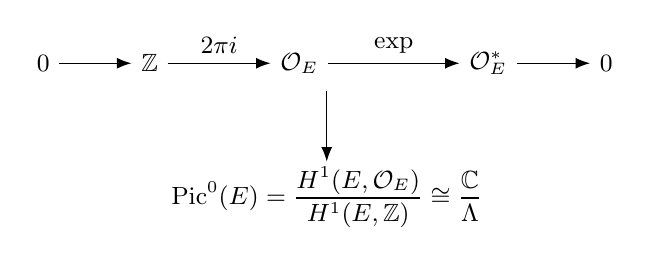
\begin{tikzpicture}[>=Latex, every node/.style={font=\small}]
    \node (z0) at (0,0) {$0$};
    \node (Z) at (1.35,0) {$\Z$};
    \node (O) at (3.25,0) {$\OO_E$};
    \node (Os) at (5.65,0) {$\OO_E^*$};
    \node (z1) at (7.15,0) {$0$};
    \draw[->, line width=0.5pt] (z0)--(Z);
    \draw[->, line width=0.5pt] (Z)--node[above] {$2\pi i$} (O);
    \draw[->, line width=0.5pt] (O)--node[above] {$\exp$} (Os);
    \draw[->, line width=0.5pt] (Os)--(z1);
    \draw[->, line width=0.5pt] (3.6,-0.35) -- (3.6,-1.25);
    \node[align=center] at (3.6,-1.7)
      {$\displaystyle \Pic^0(E)
        =\frac{H^1(E,\OO_E)}{H^1(E,\Z)}
        \cong \frac{\C}{\Lambda}$};
  \end{tikzpicture}%
}

\setlist[enumerate]{leftmargin=*, itemsep=0.35em}
\setlist[itemize]{leftmargin=*, itemsep=0.25em}
\allowdisplaybreaks
\emergencystretch=2em
\newcolumntype{L}[1]{>{\raggedright\arraybackslash}p{#1}}

\newcommand{\C}{\mathbb{C}}
\newcommand{\R}{\mathbb{R}}
\newcommand{\Z}{\mathbb{Z}}
\newcommand{\Q}{\mathbb{Q}}
\newcommand{\F}{\mathbb{F}}
\newcommand{\CP}{\mathbb{CP}}
\newcommand{\HH}{\mathbb{H}}
\newcommand{\OO}{\mathcal{O}}
\newcommand{\M}{\mathcal{M}}
\newcommand{\Div}{\operatorname{Div}}
\newcommand{\Pic}{\operatorname{Pic}}
\newcommand{\Prin}{\operatorname{Prin}}
\newcommand{\Jac}{\operatorname{Jac}}
\newcommand{\Gal}{\operatorname{Gal}}
\newcommand{\GL}{\operatorname{GL}}
\newcommand{\SL}{\operatorname{SL}}
\newcommand{\Span}{\operatorname{span}}
\newcommand{\divisor}{\operatorname{div}}
\newcommand{\ord}{\operatorname{ord}}
\newcommand{\Res}{\operatorname{Res}}
\newcommand{\degdiv}{\operatorname{deg}}
\newcommand{\rank}{\operatorname{rank}}
\newcommand{\dd}{\,d}
\newcommand{\wpprime}{\wp'}
\newcommand{\smap}{\mathfrak{s}}
\newcommand{\tate}{T_\ell E}

\declaretheorem[name=Theorem,numberwithin=chapter]{theorem}
\declaretheorem[name=Proposition,sibling=theorem]{proposition}
\declaretheorem[name=Lemma,sibling=theorem]{lemma}
\declaretheorem[name=Corollary,sibling=theorem]{corollary}
\declaretheorem[name=Definition,sibling=theorem,style=definition]{definition}
\declaretheorem[name=Example,sibling=theorem,style=definition]{example}
\declaretheorem[name=Remark,sibling=theorem,style=remark]{remark}
\declaretheorem[name=Warning,sibling=theorem,style=remark]{warningthm}
\let\warning\warningthm
\let\endwarning\endwarningthm
\declaretheorem[name=Exercise,numberwithin=chapter,style=definition]{exercise}

\newcommand{\exerciseintent}[1]{%
  \par\smallskip
  \noindent{\footnotesize\color{black!55}\emph{Intent.} #1\par}
  \smallskip
}

\newenvironment{keyidea}[1]{%
  \par\medskip
  \begin{center}
  \begin{minipage}{0.92\textwidth}
  \hrule
  \smallskip
  \textbf{#1.}\quad\ignorespaces
}{%
  \smallskip
  \hrule
  \end{minipage}
  \end{center}
  \medskip
}

\tikzset{
  arrow/.style={-{Latex[length=2mm]}, thick},
  point/.style={circle, fill=black, inner sep=1.5pt},
  labelnode/.style={font=\small, align=center},
  note/.style={draw=black!55, rounded corners=2pt, align=center, inner sep=5pt, fill=black!3},
  visualnode/.style={draw=black!60, rounded corners=2pt, align=center, inner sep=6pt, fill=black!2},
  smallvisual/.style={draw=black!60, rounded corners=2pt, align=center, inner sep=4pt, fill=black!2}
}

\crefname{warningthm}{warning}{warnings}
\Crefname{warningthm}{Warning}{Warnings}
\crefname{exercise}{exercise}{exercises}
\Crefname{exercise}{Exercise}{Exercises}


\hypersetup{
  pdftitle={Complex Tori, Jacobians, and Elliptic Curves},
  pdfsubject={The Three Faces of a Genus-One Group}
}

\begin{document}

\frontmatter
\raggedbottom
\begin{titlepage}
\thispagestyle{empty}
\centering
\vspace*{0.08\textheight}

{\large\scshape A Textbook for Complex Analysis and Genus One\par}

\vspace{1.25cm}
\rule{0.74\textwidth}{0.45pt}\par
\vspace{0.85cm}

{\Huge\bfseries Complex Tori, Jacobians,\\[0.25em]
and Elliptic Curves\par}

\vspace{0.55cm}
{\Large\itshape The Three Faces of a Genus-One Group\par}

\vspace{0.85cm}
\rule{0.74\textwidth}{0.45pt}\par

\vspace{1.35cm}
\begin{minipage}{0.74\textwidth}
\centering
Complex tori, degree-zero divisor classes, and plane cubics as one genus-one
group:
\[
  \C/\Lambda\;\cong\;\Pic^0(E)\;\cong\;E(\C)
\]
as complex Lie groups.  The chord--tangent law is torus addition transported by
\[
  z\longmapsto[\wp(z):\wp'(z):1].
\]
\end{minipage}

\vfill
{\large Spring 2026\par}
\vspace{0.45cm}
{\small\scshape Riemann Surfaces and Complex Analysis\par}
\end{titlepage}

\chapter*{Preface}
\addcontentsline{toc}{chapter}{Preface}

This textbook develops the genus-one bridge between complex analysis, Riemann
surface theory, and the algebraic geometry of plane cubics.  Its main purpose is
to explain why the complex torus, the Jacobian, and the smooth cubic are three
presentations of one mathematical object.

The organizing claim is simple to state.  A lattice \(\Lambda\subset\C\) gives a
compact complex Lie group \(T=\C/\Lambda\).  The Weierstrass functions attach to
it a smooth cubic
\[
  E:\quad Y^2Z=4X^3-g_2XZ^2-g_3Z^3,
\]
and the map \(z\mapsto[\wp(z):\wp'(z):1]\) identifies \(T\) with \(E(\C)\).
Divisors identify the same group with \(\Pic^0(E)\).  Under this identification,
the geometric chord--tangent rule on \(E\) is just addition on the torus.

The book starts from the exam material: differential forms, Stokes' theorem,
residues, compact Riemann surfaces, divisors, and Riemann--Roch.  Those topics
are not reviewed as a checklist; they are used as the mechanism that makes the
main theorem natural.

\chapter*{Big Picture}
\addcontentsline{toc}{chapter}{Big Picture}
\label{front:big-picture}

The goal of this book is to understand one object from three directions.  The
object is a genus-one complex group.  It first appears analytically as a quotient
\[
  T=\C/\Lambda,
\]
where addition is inherited from addition in \(\C\).  It then appears
geometrically as a Jacobian,
\[
  \Pic^0(E),
\]
where the group law is encoded by degree-zero divisor classes.  Finally it
appears algebraically as the complex points of a smooth plane cubic,
\[
  E(\C):\quad Y^2Z=4X^3-g_2XZ^2-g_3Z^3.
\]

\begin{center}
\resizebox{0.82\linewidth}{!}{\classicTrinityDiagram}
\end{center}

\noindent
The central theorem says that these are not merely related examples:
\[
  \C/\Lambda \cong \Pic^0(E) \cong E(\C)
\]
as complex Lie groups.  This phrase is important: the maps are both
biholomorphic and compatible with the group laws.  Thus the statement is
stronger than an isomorphism of abstract abelian groups; it also preserves the
complex structure.  The most visible consequence is the chord--tangent law.  On
the torus, addition is simply
\[
  [u]+[v]=[u+v].
\]
On the cubic, the same addition is disguised as a geometric recipe: draw the line
through two points, take the third intersection with the cubic, and reflect it.

\section*{What Must Be Understood}

\begin{enumerate}
\item \textbf{Why a torus is a Riemann surface.}
  A lattice quotient \(\C/\Lambda\) is compact, genus one, and still carries a
  holomorphic group law.

\item \textbf{Why elliptic functions are constrained.}
  Meromorphic periodic functions cannot have arbitrary zeros and poles.  The
  residue theorem and the argument principle force balancing laws.

\item \textbf{Why the Weierstrass function creates a cubic.}
  The functions \(\wp\) and \(\wp'\) satisfy
  \[
    \wp'^2=4\wp^3-g_2\wp-g_3,
  \]
  so \(z\mapsto[\wp(z):\wp'(z):1]\) sends the torus into a plane cubic.

\item \textbf{Why divisors produce the Jacobian.}
  Principal divisors have degree zero, and Abel's theorem says that on a torus a
  degree-zero divisor is principal exactly when its Abel sum vanishes.

\item \textbf{Why Riemann--Roch gives the correct coordinates.}
  On a genus-one surface, \(\ell(nO)=n\).  Thus \(1,\wp,\wp'\) are exactly the
  three functions needed to map the torus into \(\CP^2\).

\item \textbf{Why line intersection becomes addition.}
  A line meeting the cubic in \(P,Q,R\) cuts out a principal divisor
  \([P]+[Q]+[R]-3[O]\).  Abel's theorem converts this into the group equation
  \(P+Q+R=O\), so the sum of \(P\) and \(Q\) is the reflection of \(R\).
\end{enumerate}

\begin{keyidea}{The route through the book}
The chapters move from the exam tools to the torus, from the torus to elliptic
functions, from elliptic functions to the cubic, and from divisors to the
Jacobian.  The final synthesis is that the analytic, geometric, and algebraic
constructions describe the same group.
\end{keyidea}

\chapter*{Notation}
\addcontentsline{toc}{chapter}{Notation}
\label{front:notation}

\begin{center}
\begin{tabular}{@{}ll@{}}
\(\C,\R,\Z,\Q,\F_p\) & complex, real, integer, rational, and finite fields\\
\(\HH\) & upper half-plane\\
\(\Lambda\) & lattice \(\Z\omega_1+\Z\omega_2\)\\
\(T=\C/\Lambda\) & complex torus\\
\(O\) & identity of \(T\), also point at infinity of \(E\)\\
\(\wp,\wp'\) & Weierstrass function and derivative\\
\(g_2,g_3,\Delta\) & invariants and discriminant \(g_2^3-27g_3^2\)\\
\(E\) & cubic \(Y^2Z=4X^3-g_2XZ^2-g_3Z^3\)\\
\(\Div(X)\) & divisor group of \(X\)\\
\(\divisor(f)\) & principal divisor of \(f\)\\
\(\Pic^0(X)\) & degree-zero divisor classes modulo principal divisors\\
\(\smap\) & Abel--Jacobi sum map\\
\(L(D),\ell(D)\) & meromorphic functions bounded by \(D\), and its dimension\\
\(\Phi\) & Weierstrass map \([\wp:\wp':1]\)\\
\(\oplus\) & transported group law on \(E\)\\
\(\boxplus\) & chord--tangent construction\\
\(j\) & \(j\)-invariant \(1728g_2^3/\Delta\)\\
\end{tabular}
\end{center}

\noindent
The symbols in this table are used throughout the book.  Later chapters refine
some definitions, but this front-matter list fixes the basic notation before the
main exposition begins.

\chapter*{Course Guide}
\addcontentsline{toc}{chapter}{Course Guide}
\label{front:syllabus}

\section*{Aim of the Course}
\addcontentsline{toc}{section}{Aim of the Course}

This twelve-week course gives a route through the book for one two-hour lecture
each week.  The goal is not to survey elliptic curves broadly, but to understand
one central identification in detail:
\[
  \C/\Lambda \;\cong\; \Pic^0(E) \;\cong\; E(\C).
\]
Here the isomorphisms are isomorphisms of complex Lie groups.  The course ends
by proving that the chord--tangent law on a smooth plane cubic is addition on
the torus transported by
\[
  z\longmapsto[\wp(z):\wp'(z):1].
\]

\section*{Prerequisites}
\addcontentsline{toc}{section}{Prerequisites}

The course assumes a first course in complex analysis.  The following table
separates what is used immediately from what the text develops during the
course.

\begin{center}
\small
\renewcommand{\arraystretch}{1.18}
\begin{tabular}{@{}L{0.24\linewidth}L{0.64\linewidth}@{}}
\textbf{Assumed} &
Holomorphic functions, contour integration, residues, isolated singularities,
and basic topology of subsets of \(\C\).\\
\textbf{Reviewed as needed} &
Differential forms, Stokes' theorem, meromorphic functions on compact surfaces,
and zero-pole counting.\\
\textbf{Developed carefully} &
Compact Riemann surfaces, divisors, Picard groups, Jacobians,
genus-one Riemann--Roch, and the Weierstrass embedding.
\end{tabular}
\end{center}

\section*{Structure of the Course}
\addcontentsline{toc}{section}{Structure of the Course}

\begin{center}
\small
\renewcommand{\arraystretch}{1.22}
\begin{tabular}{@{}L{0.11\linewidth}L{0.23\linewidth}L{0.27\linewidth}L{0.27\linewidth}@{}}
\textbf{Weeks} & \textbf{Theme} & \textbf{Main objects} & \textbf{Question}\\
\hline
1--3 &
Analytic foundations &
Forms, residues, compact surfaces, lattices &
How does complex analysis produce a compact genus-one group?\\
4--6 &
Elliptic functions &
Periodic meromorphic functions, \(\wp\), principal divisors &
How do functions on \(\C/\Lambda\) remember the group law?\\
7--9 &
Divisors and Jacobians &
\(L(D)\), \(\Pic^0(E)\), Abel--Jacobi, \([\wp:\wp':1]\) &
Why does the analytic torus become a smooth plane cubic?\\
10--12 &
The cubic group law &
Lines, tangents, Abel's theorem, \(j\)-invariant &
Why is chord--tangent addition the same operation as torus addition?
\end{tabular}
\end{center}

\section*{Weekly Lecture Plan}
\addcontentsline{toc}{section}{Weekly Lecture Plan}

\begin{center}
\footnotesize
\renewcommand{\arraystretch}{1.16}
\begin{tabular}{@{}L{0.06\linewidth}L{0.31\linewidth}L{0.15\linewidth}L{0.36\linewidth}@{}}
\textbf{Week} & \textbf{Lecture focus} & \textbf{Reading} & \textbf{Core result}\\
\hline
1 &
Forms, residues, and global obstructions &
Ch. 1; App. A &
Residues turn local singular data into a global constraint.\\
2 &
Compact Riemann surfaces and genus &
Ch. 2 &
Compactness changes complex analysis from local function theory into global
geometry.\\
3 &
Lattices and complex tori &
Ch. 3 &
\(\C/\Lambda\) is a compact genus-one Riemann surface and a complex Lie group.\\
4 &
Elliptic functions &
Ch. 4 &
Zeros, poles, and residues of elliptic functions balance on a fundamental
parallelogram.\\
5 &
The Weierstrass \(\wp\)-function &
Ch. 5 &
\(\wp\) and \(\wp'\) satisfy
\(\wp'^2=4\wp^3-g_2\wp-g_3\).\\
6 &
Divisors and principal divisors &
Ch. 6 &
Zeros and poles become degree-zero divisor classes modulo principal divisors.\\
7 &
Riemann--Roch in genus one &
Ch. 7 &
\(\ell(nO)=n\) for \(n\geq 1\), giving the functions needed for the cubic map.\\
8 &
Abel's theorem and the Jacobian &
Ch. 8 &
The map \(P\mapsto[P]-[O]\) identifies \(E\) with \(\Pic^0(E)\) as complex Lie
groups.\\
9 &
The Weierstrass embedding &
Ch. 9 &
\(1,\wp,\wp'\) embed the torus into \(\CP^2\) as a smooth cubic.\\
10 &
The plane cubic group law &
Ch. 10 &
Three collinear points on the cubic have sum \(O\).\\
11 &
Transport of addition &
Ch. 11; Ch. 14 &
The chord--tangent operation is torus addition transported by
\([\wp:\wp':1]\).\\
12 &
Synthesis and further directions &
Chs. 12--14 &
Cohomology, moduli, the \(j\)-invariant, and finite-field questions extend the
same genus-one structure.
\end{tabular}
\end{center}

\section*{Exercises and Written Work}
\addcontentsline{toc}{section}{Exercises and Written Work}

Exercises are meant to force translation between the analytic, divisor-theoretic,
and geometric languages.  They should be attempted before consulting the
solutions appendix.

\begin{center}
\small
\renewcommand{\arraystretch}{1.2}
\begin{tabular}{@{}L{0.22\linewidth}L{0.48\linewidth}L{0.18\linewidth}@{}}
\textbf{Work} & \textbf{Main task} & \textbf{Due}\\
\hline
Problem Set 1 &
Residues, compactness, genus, and quotient tori &
After Week 3\\
Problem Set 2 &
Elliptic functions, \(\wp\), and principal divisors &
After Week 6\\
Problem Set 3 &
Riemann--Roch, Abel--Jacobi, and the Weierstrass embedding &
After Week 9\\
Problem Set 4 &
Line divisors, tangents, and transported addition &
After Week 11\\
Final synthesis &
A concise proof narrative of
\(\C/\Lambda\cong\Pic^0(E)\cong E(\C)\) as complex Lie groups &
Week 12
\end{tabular}
\end{center}

\begin{keyidea}{Final target}
By the end of the course, the student should be able to read the equation of
the Weierstrass cubic, the divisor class \([P]-[O]\), and the point
\(z\in\C/\Lambda\) as three notations for the same genus-one group element.
\end{keyidea}

\tableofcontents

\mainmatter
\flushbottom

\chapter[Exam Background]{Exam Background: Forms, Residues, and Global Obstructions}
\label{ch:exam-background}

The main theorem concerns a torus, a Jacobian, and a cubic.  The proof begins
much earlier, with a lesson from the midterm: a local calculation can fail
globally because a differential form carries an obstruction.
The winding form on \(\R^2\setminus\{0\}\),
\[
  \omega_{\mathrm{wind}}=\frac{-y\,dx+x\,dy}{x^2+y^2},
\]
is closed, but \(\int_{S^1}\omega_{\mathrm{wind}}=2\pi\).  It is locally
\(d\theta\), but no global single-valued angle function exists.

\begin{definition}
An obstruction is a locally invisible quantity that is detected by integration
around a global cycle.  In complex analysis the model obstruction is the residue:
\[
  \frac{1}{2\pi i}\int_\gamma \frac{f'(z)}{f(z)}\,dz.
\]
\end{definition}

The same idea drives the later theory of divisors.  Zeros and poles of a
meromorphic function are local data.  On a compact surface they cannot be chosen
freely, because residues and periods force global balancing laws.

\begin{proposition}[The exam mechanism]
\label{prop:exam-mechanism}
The sequence
\[
  \text{forms} \longrightarrow \text{Stokes} \longrightarrow
  \text{residues} \longrightarrow \text{global constraints}
\]
is the mechanism behind the divisor statements used later.
\end{proposition}

\begin{proof}
Stokes' theorem turns the integral of an exact form over a boundary into an
interior integral.  If a meromorphic form is regular except at finitely many
points, deleting small disks around those points makes Stokes applicable.  Letting
the disk radii shrink leaves only small circle integrals, hence residues.  On a
compact surface the outer boundary is absent, so the sum of all local residues
must vanish.
\end{proof}

\begin{keyidea}{Why this matters}
The statement that principal divisors have degree zero is the divisor version of
the residue theorem applied to \(df/f\).  Abel's theorem is a refined version:
not only the total number of zeros and poles but also their Abel sum is
constrained.
\end{keyidea}

\section*{Exercises}
\addcontentsline{toc}{section}{Exercises}

\exerciseintent{Check, by direct differentiation, that the local winding form is closed away from its singularity.}
\begin{exercise}
Write \(\omega_{\mathrm{wind}}=P\,dx+Q\,dy\).  Compute \(Q_x\), compute
\(P_y\), and subtract them to verify directly that
\[
  d\omega_{\mathrm{wind}}=(Q_x-P_y)\,dx\wedge dy=0
\]
on \(\R^2\setminus\{0\}\).
\end{exercise}

\exerciseintent{Compute the period of the winding form on the basic loop and see the obstruction to exactness.}
\begin{exercise}
Parametrize the unit circle by \(x=\cos t\), \(y=\sin t\).  Compute \(dx\),
\(dy\), the numerator \(-y\,dx+x\,dy\), and then the integral
\(\int_{S^1}\omega_{\mathrm{wind}}\).
\end{exercise}

\exerciseintent{Relate the local order of a meromorphic function to the residue of its logarithmic derivative.}
\begin{exercise}
Let \(f\) be meromorphic near \(p\).  Write \(f=(z-p)^m u(z)\) with
\(u(p)\ne0\).  Compute \(df/f\) explicitly and read off the coefficient of
\((z-p)^{-1}\,dz\), showing that it is \(\ord_p(f)\).
\end{exercise}

\exerciseintent{Turn the compact residue theorem into the degree-zero property of principal divisors.}
\begin{exercise}
Assume \(X\) is compact and \(f\) is a nonzero meromorphic function on \(X\).
Compute
\[
  \sum_p\Res_p(df/f)
\]
in two ways: first by the compact residue theorem, and second using the previous
exercise.  Conclude that \(\degdiv\divisor(f)=0\).
\end{exercise}

\chapter{Compact Riemann Surfaces and Genus}
\label{ch:riemann-surfaces}

A Riemann surface is the natural setting for one-variable complex analysis after
we stop insisting that all functions live on open subsets of \(\C\).  It is a
topological surface with charts to \(\C\) whose transition functions are
holomorphic.  Compact Riemann surfaces are the complex-analytic analogues of
closed algebraic curves.

\begin{definition}
A compact Riemann surface \(X\) has genus \(g\) if its underlying oriented
topological surface has \(g\) handles.  Equivalently,
\(\chi(X)=2-2g\).
\end{definition}

The midterm computation that the real torus has Euler characteristic \(0\) is
therefore already telling us that a complex torus has genus \(1\).  This number is
not cosmetic.  It is exactly the number that makes Riemann--Roch read
\(\ell(D)=\deg D\) for positive divisors on an elliptic curve.

\begin{proposition}
\label{prop:compact-functions}
Every holomorphic function on a compact connected Riemann surface is constant.
\end{proposition}

\begin{proof}
The image of a compact surface under a holomorphic function is compact in \(\C\),
so the function has a maximum absolute value.  The maximum modulus principle then
forces the function to be locally constant, hence constant.
\end{proof}

\begin{definition}
A meromorphic function on a Riemann surface is a holomorphic map to
\(\CP^1\).  Its poles are the points mapping to \(\infty\).
\end{definition}

\begin{keyidea}{Compactness changes the rules}
On a compact surface, nonconstant holomorphic functions disappear, but
meromorphic functions become structured maps to \(\CP^1\).  The map
\(\wp:T\to\CP^1\) is exactly such a map.
\end{keyidea}

\section*{Exercises}
\addcontentsline{toc}{section}{Exercises}

\exerciseintent{Convert Euler characteristic into genus in the genus-one case.}
\begin{exercise}
Substitute \(\chi=0\) into \(\chi=2-2g\) and solve the resulting linear equation
for \(g\).
\end{exercise}

\exerciseintent{Identify exactly where compactness enters the maximum modulus argument.}
\begin{exercise}
Use the concrete function \(f(z)=z\) on \(\C\).  Compute why \(|f|\) has no
maximum on \(\C\), and use this calculation to identify the step in the maximum
modulus proof that fails on noncompact surfaces.
\end{exercise}

\exerciseintent{Use compactness and local normal forms to prove zeros and poles are finite.}
\begin{exercise}
Suppose a meromorphic function on a compact surface had infinitely many zeros or
poles.  Use compactness to produce an accumulation point, then use the local
forms \((z-p)^m u(z)\) and \((z-p)^{-m}u(z)\) to compute why this contradicts
isolation of zeros and poles.
\end{exercise}

\exerciseintent{Recover the torus genus by a concrete cell count on the glued parallelogram.}
\begin{exercise}
The quotient of a parallelogram by identifying opposite sides is a topological
torus.  Count the cell classes \(F,E,V\) after the identifications, compute
\[
  \chi=F-E+V,
\]
and then use \(\chi=2-2g\) to compute the genus.
\end{exercise}

\chapter{Lattices and Complex Tori}
\label{ch:lattices-tori}

Let \(\omega_1,\omega_2\in\C\) be real-linearly independent.  The lattice
\[
  \Lambda=\Z\omega_1+\Z\omega_2
\]
tiles the complex plane by translates of a parallelogram.  The quotient
\[
  T=\C/\Lambda
\]
is obtained by identifying points that differ by lattice elements.

\begin{definition}
The complex torus associated to \(\Lambda\) is the quotient group
\(T=\C/\Lambda\), equipped with the complex structure induced from small disks in
\(\C\).
\end{definition}

Addition in \(\C\) descends to addition on \(T\):
\[
  [u]+[v]=[u+v].
\]
This is the analytic group law.  It is associative, commutative, and has identity
\([0]\) because those facts were true before quotienting.

\begin{proposition}
\label{prop:torus-surface}
The quotient \(T=\C/\Lambda\) is a compact genus-one Riemann surface and a
complex Lie group.
\end{proposition}

\begin{proof}
A fundamental parallelogram is compact, and its quotient maps onto \(T\), so
\(T\) is compact.  Away from identified boundary points, charts come directly
from the plane; near a boundary identification one takes a small disk whose
translates are disjoint and uses its projection.  The quotient of a parallelogram
by opposite-side identifications is a topological torus, hence genus one.
Addition is holomorphic because it is induced by the holomorphic addition map on
\(\C\).
\end{proof}

\begin{center}
\begin{tikzpicture}[scale=0.65]
  \begin{scope}
    \drawprecisetorus
  \end{scope}
  \node[align=center, font=\small] at (0,-3.15)
    {A real picture of the quotient surface.\\The complex structure comes from
    the plane before gluing.};
\end{tikzpicture}
\end{center}

\section*{Exercises}
\addcontentsline{toc}{section}{Exercises}

\exerciseintent{Verify that addition on the quotient is independent of chosen representatives.}
\begin{exercise}
Let \(u'=u+\lambda\) and \(v'=v+\mu\) with \(\lambda,\mu\in\Lambda\).  Compute
\(u'+v'\) and show explicitly that it differs from \(u+v\) by an element of
\(\Lambda\).  Conclude that addition on \(\C/\Lambda\) is well-defined.
\end{exercise}

\exerciseintent{Check that an integral change of basis preserves the same lattice.}
\begin{exercise}
Let
\[
  \begin{pmatrix}\omega'_1\\ \omega'_2\end{pmatrix}
  =
  A\begin{pmatrix}\omega_1\\ \omega_2\end{pmatrix},
  \qquad A\in\GL_2(\Z).
\]
Use the integer entries of \(A\) and \(A^{-1}\) to prove by direct inclusion
that \(\Z\omega_1+\Z\omega_2=\Z\omega'_1+\Z\omega'_2\).
\end{exercise}

\exerciseintent{Normalize a lattice basis so its period ratio lies in the upper half-plane.}
\begin{exercise}
Let \(\tau=\omega_2/\omega_1\).  First compute why \(\operatorname{Im}\tau\ne0\).
If \(\operatorname{Im}\tau<0\), swap the basis vectors and compute
\(\operatorname{Im}(1/\tau)\).  Conclude that an oriented basis can be chosen
with \(\tau\in\HH\).
\end{exercise}

\exerciseintent{Check that torus translations are well-defined biholomorphic group translations.}
\begin{exercise}
Let \(a\in\C\).  Show that the translation map
\[
  T\longrightarrow T,\qquad [z]\longmapsto [z+a]
\]
is a well-defined biholomorphic group translation by computing what happens when
\(z\) is replaced by \(z+\lambda\), and by writing down the inverse translation.
\end{exercise}

\exerciseintent{Separate complex Lie group isomorphism from a mere abstract group isomorphism.}
\begin{exercise}
In the final theorem, the symbol \(\cong\) means isomorphism of complex Lie
groups.  Make a three-row checklist: group homomorphism, holomorphic map, and
holomorphic inverse.  For each row, write the equation or property that must be
verified beyond an abstract abelian-group isomorphism.
\end{exercise}

\chapter{Elliptic Functions on \texorpdfstring{\(\C/\Lambda\)}{C/Lambda}}
\label{ch:elliptic-functions}

A meromorphic function on \(T=\C/\Lambda\) is the same thing as a meromorphic
function \(f\) on \(\C\) satisfying \(f(z+\lambda)=f(z)\) for every
\(\lambda\in\Lambda\).  Such functions are called elliptic functions.

\begin{definition}
An elliptic function for \(\Lambda\) is a meromorphic function
\(f:\C\to\CP^1\) that is \(\Lambda\)-periodic.
\end{definition}

Compactness immediately rules out holomorphic examples.

\begin{proposition}
\label{prop:no-holomorphic-elliptic}
A holomorphic elliptic function is constant.
\end{proposition}

\begin{proof}
It descends to a holomorphic function on the compact surface \(T\), so
\cref{prop:compact-functions} applies.
\end{proof}

The useful elliptic functions must therefore have poles.  The exam residue
method now gives three constraints.  In one period parallelogram, an elliptic
function has residue sum zero, as many zeros as poles counted with multiplicity,
and the weighted sum of its zeros minus the weighted sum of its poles lies in
\(\Lambda\).

\begin{theorem}[Elliptic Liouville laws]
\label{thm:elliptic-liouville}
Let \(f\) be a nonzero elliptic function.  In a fundamental parallelogram avoiding
zeros and poles on its boundary,
\[
  \sum \Res(f\,dz)=0,\qquad
  \sum \ord_a(f)=0,\qquad
  \sum_{\ord_a(f)>0}\ord_a(f)a-\sum_{\ord_b(f)<0}(-\ord_b(f))b\in\Lambda .
\]
\end{theorem}

\begin{proof}[Proof sketch]
Integrate \(f\,dz\), \(f'/f\,dz\), and \(z f'/f\,dz\) around the boundary of a
period parallelogram.  Periodicity makes opposite sides cancel in the first two
integrals.  In the third integral, opposite sides cancel up to periods, which is
why the final answer is only well-defined modulo \(\Lambda\).
\end{proof}

\begin{keyidea}{The bridge to Abel}
The third law is already Abel's theorem in its torus form: a principal divisor of
degree zero has Abel sum zero in \(\C/\Lambda\).
\end{keyidea}

\section*{Exercises}
\addcontentsline{toc}{section}{Exercises}

\exerciseintent{Use the residue obstruction to rule out a single simple pole on a torus.}
\begin{exercise}
Assume a nonconstant elliptic function has total pole order \(1\).  Write the
Laurent expansion at its unique simple pole, compute the residue contribution,
and use the residue-sum law to obtain a contradiction.  Conclude that the total
pole order is at least \(2\).
\end{exercise}

\exerciseintent{Compute boundary cancellation on a period parallelogram via the argument principle.}
\begin{exercise}
Apply the argument principle on a fundamental parallelogram \(P\):
\[
  \frac{1}{2\pi i}\int_{\partial P}\frac{f'}{f}\,dz.
\]
Pair the four side integrals using periodicity and compute why the total is
\(0\).  Conclude that the number of zeros equals the number of poles, counted
with multiplicity.
\end{exercise}

\exerciseintent{See why Abel sums naturally live modulo the lattice.}
\begin{exercise}
Let a lift \(a_i\in\C\) of a point of \(T\) be replaced by \(a_i+\lambda_i\),
with \(\lambda_i\in\Lambda\).  Compute how
\(\sum_i m_i a_i\) changes, and conclude that the Abel sum is naturally a point
of \(\C/\Lambda\), not of \(\C\).
\end{exercise}

\exerciseintent{Verify the descent/ascent between elliptic functions and meromorphic functions on the quotient.}
\begin{exercise}
Let \(q:\C\to T=\C/\Lambda\) be the quotient map.  Show that a meromorphic
function \(F\) on \(T\) pulls back to an elliptic function by computing
\((F\circ q)(z+\lambda)\).  Conversely, if \(f(z+\lambda)=f(z)\), compute why
the formula \(F([z])=f(z)\) is independent of the chosen representative.
\end{exercise}

\exerciseintent{Compute an explicit principal-divisor Abel sum and connect it to \(\smap(\divisor(f))=0\).}
\begin{exercise}
Let \(f\) be a nonzero elliptic function with divisor
\[
  \divisor(f)=[a_1]+[a_2]-[b_1]-[b_2]
\]
on \(T\), with chosen lifts \(a_1,a_2,b_1,b_2\in\C\).  Use the third identity
in \cref{thm:elliptic-liouville} to compute
\[
  a_1+a_2-b_1-b_2\pmod{\Lambda}.
\]
Then rewrite the calculation as \(\smap(\divisor(f))=0\).
\end{exercise}

\chapter{The Weierstrass \texorpdfstring{\(\wp\)}{wp}-Function}
\label{ch:weierstrass-wp}

The analytic theory of elliptic curves centers on the Weierstrass function
\[
  \wp(z)=\frac{1}{z^2}+
  \sum_{\lambda\in\Lambda\setminus\{0\}}
  \left(\frac{1}{(z-\lambda)^2}-\frac{1}{\lambda^2}\right).
\]
The subtraction term makes the series converge normally on compact sets away from
\(\Lambda\).  The function is even, \(\Lambda\)-periodic, and has one double pole
per fundamental parallelogram.

\begin{definition}
The Eisenstein series of weight \(k\) is
\[
  G_k(\Lambda)=\sum_{\lambda\in\Lambda\setminus\{0\}}\lambda^{-k}
\]
for \(k>2\).  Set \(g_2=60G_4\) and \(g_3=140G_6\).
\end{definition}

\begin{theorem}[The differential equation]
\label{thm:wp-ode-new}
The Weierstrass function satisfies
\[
  \wp'(z)^2=4\wp(z)^3-g_2\wp(z)-g_3.
\]
\end{theorem}

\begin{proof}[Proof sketch]
Compare Laurent expansions at \(0\).  Both sides have principal part
\(4z^{-6}\), and the constants \(g_2,g_3\) are chosen so that the remaining
negative and constant terms cancel.  The difference is then a holomorphic
elliptic function, hence constant by \cref{prop:no-holomorphic-elliptic}; its
Laurent expansion shows that constant is \(0\).
\end{proof}

\begin{corollary}
The functions \(x=\wp(z)\) and \(y=\wp'(z)\) land on the affine cubic
\[
  y^2=4x^3-g_2x-g_3.
\]
\end{corollary}

This is the exact moment where the analytic face becomes algebraic.  The final
exam's minimal-polynomial problem for \(\wp'\) over \(\C(\wp)\) is the algebraic
shadow of this differential equation.

\section*{Exercises}
\addcontentsline{toc}{section}{Exercises}

\exerciseintent{Prove evenness of \(\wp\) by reindexing the defining lattice sum.}
\begin{exercise}
Use the defining lattice sum for \(\wp\).  Substitute \(-z\) for \(z\), then
reindex the lattice terms by \(\lambda\mapsto-\lambda\) to show by calculation
that \(\wp(-z)=\wp(z)\).
\end{exercise}

\exerciseintent{Use the chain rule to derive the oddness of \(\wp'\).}
\begin{exercise}
Differentiate the identity \(\wp(-z)=\wp(z)\) with respect to \(z\).  Keep track
of the chain-rule minus sign and compute the resulting parity of \(\wp'\).
\end{exercise}

\exerciseintent{Read the Weierstrass differential equation as algebraicity over \(\C(\wp)\).}
\begin{exercise}
Assuming \cref{thm:wp-ode-new}, write an explicit quadratic polynomial
\[
  Y^2-(4\wp^3-g_2\wp-g_3)\in \C(\wp)[Y]
\]
that is satisfied by \(Y=\wp'\).  Use this calculation to show that \(\wp'\) is
algebraic of degree at most \(2\) over \(\C(\wp)\).
\end{exercise}

\exerciseintent{Extract the pole orders that will feed the genus-one Riemann--Roch calculation.}
\begin{exercise}
Using the Laurent expansions
\[
  \wp(z)=z^{-2}+O(z^2),\qquad \wp'(z)=-2z^{-3}+O(z),
\]
compute the pole orders of \(\wp\) and \(\wp'\) at \(O\in T\).
\end{exercise}

\exerciseintent{Substitute the Weierstrass functions into the cubic equation.}
\begin{exercise}
Set \(x=\wp(z)\) and \(y=\wp'(z)\).  Substitute these expressions into
\cref{thm:wp-ode-new} and verify directly that the pair \((x,y)\) lies on the
affine cubic
\[
  y^2=4x^3-g_2x-g_3.
\]
\end{exercise}


\chapter{Divisors and Principal Divisors}
\label{ch:divisors}

A divisor records zeros and poles as a formal integer combination of points.

\begin{definition}
For a compact Riemann surface \(X\), a divisor is a finite sum
\[
  D=\sum n_p[p],\qquad n_p\in\Z.
\]
Its degree is \(\degdiv D=\sum n_p\).  If \(f\) is meromorphic, its principal
divisor is
\[
  \divisor(f)=\sum_p \ord_p(f)[p].
\]
\end{definition}

Principal divisors are the geometric version of logarithmic derivatives.  Since
\(\Res_p(df/f)=\ord_p(f)\), the compact residue theorem gives:

\begin{proposition}
\label{prop:principal-degree-zero}
Every principal divisor on a compact Riemann surface has degree zero.
\end{proposition}

\begin{proof}
The meromorphic one-form \(df/f\) has residue \(\ord_p(f)\) at \(p\).  The sum of
residues on a compact Riemann surface is zero, so
\(\degdiv\divisor(f)=0\).
\end{proof}

\begin{definition}
The degree-zero divisor group is \(\Div^0(X)\).  The principal divisors form a
subgroup \(\Prin(X)\subset\Div^0(X)\), and
\[
  \Pic^0(X)=\Div^0(X)/\Prin(X).
\]
\end{definition}

The group \(\Pic^0(E)\) is not decorative notation.  It is the geometric home of
the same group already seen analytically as \(\C/\Lambda\).  A point \([P]-[O]\)
is a degree-zero divisor class, and the map \(P\mapsto[P]-[O]\) will identify the
curve with its Jacobian.

\section*{Exercises}
\addcontentsline{toc}{section}{Exercises}

\exerciseintent{Practice divisor bookkeeping, including the contribution at infinity.}
\begin{exercise}
Compute the divisor of \(z^2(z-1)^{-3}\) on \(\CP^1\).  First compute the
orders at \(0\) and \(1\).  Then use the coordinate \(w=1/z\) to compute the
order at \(\infty\).
\end{exercise}

\exerciseintent{Verify that principal divisors form a degree-zero subgroup.}
\begin{exercise}
For meromorphic functions \(f,g\), compute \(\divisor(fg)\),
\(\divisor(f^{-1})\), and \(\divisor(c)\) for \(c\in\C^*\).  Use these
calculations, together with degree zero for principal divisors, to show that
\(\Prin(X)\) is a subgroup of \(\Div^0(X)\).
\end{exercise}

\exerciseintent{Check the basic degree-zero divisor attached to a pointed curve.}
\begin{exercise}
Compute the degree of \([P]-[O]\) by adding its two coefficients.
\end{exercise}

\exerciseintent{Compute addition of degree-zero divisor classes in \(\Pic^0\).}
\begin{exercise}
Show that
\[
  ([P]-[O])+([Q]-[O])=[P]+[Q]-2[O]
\]
defines an element of \(\Pic^0(X)\) by explicitly computing the degree of the
right-hand side and then passing modulo \(\Prin(X)\).
\end{exercise}

\exerciseintent{Translate equality in \(\Pic^0\) into a principal-divisor condition.}
\begin{exercise}
Let \(D,D'\in\Div^0(X)\).  Compute the difference \(D-D'\) in the quotient
\(\Div^0(X)/\Prin(X)\).  State and prove the criterion for \(D\) and \(D'\) to
define the same element of \(\Pic^0(X)\).
\end{exercise}

\chapter{Riemann--Roch in Genus One}
\label{ch:riemann-roch}

For a divisor \(D\), define
\[
  L(D)=\{f\in\M(X): \divisor(f)+D\ge 0\}\cup\{0\}.
\]
Thus \(L(D)\) is the vector space of meromorphic functions whose poles are bounded
by \(D\).

\begin{theorem}[Riemann--Roch]
\label{thm:rr}
On a compact Riemann surface of genus \(g\),
\[
  \ell(D)-\ell(K-D)=\degdiv D+1-g,
\]
where \(K\) is a canonical divisor and \(\ell(D)=\dim_\C L(D)\).
\end{theorem}

We will use the theorem in its genus-one form.  On a complex torus, \(dz\) is a
nowhere-vanishing holomorphic \(1\)-form, so \(K\sim0\).  Since \(g=1\), the
formula becomes
\[
  \ell(D)-\ell(-D)=\degdiv D.
\]
If \(\deg D>0\), then \(L(-D)=0\), and therefore \(\ell(D)=\deg D\).

\begin{corollary}
\label{cor:ell-nO}
For \(T=\C/\Lambda\) and \(O=[0]\),
\[
  \ell(nO)=n\qquad(n\ge 1).
\]
\end{corollary}

This is the dimension count behind the fact that \(1,\wp,\wp'\) span \(L(3O)\).
The function \(1\) has no pole, \(\wp\) has a
double pole at \(O\), and \(\wp'\) has a triple pole at \(O\).  Since
\(\ell(3O)=3\), these three functions exhaust the space.

\begin{warning}
Riemann--Roch is a deep theorem in general.  In this book it is used as a
standard final-exam tool and interpreted carefully in genus one.  Claims that
require more algebraic geometry are explicitly labeled as such.
\end{warning}

\section*{Exercises}
\addcontentsline{toc}{section}{Exercises}

\exerciseintent{Use genus-one Riemann--Roch as a dimension calculator.}
\begin{exercise}
Using \(\ell(nO)=n\), compute \(\dim L(O)\), \(\dim L(2O)\), and
\(\dim L(3O)\) by substituting \(n=1,2,3\).
\end{exercise}

\exerciseintent{Show why \(L(O)\) contains no nonconstant function.}
\begin{exercise}
Split into two cases.  If \(f\in L(O)\) has no pole, use compactness to compute
that it is constant.  If \(f\) has a simple pole at \(O\), compute its total
pole order and compare with the elliptic-function pole-order obstruction from
Chapter 4.
\end{exercise}

\exerciseintent{Use pole orders to prove linear independence of \(1,\wp,\wp'\).}
\begin{exercise}
Suppose \(a+b\wp+c\wp'=0\).  Compare the pole orders \(0,2,3\) at \(O\) and use
the largest pole order term to compute successively that \(c=b=a=0\).
\end{exercise}

\exerciseintent{Combine membership, pole-order independence, and dimension to identify \(L(2O)\).}
\begin{exercise}
Use \(\ell(2O)=2\) and the pole order of \(\wp\) to prove
\[
  L(2O)=\Span_\C(1,\wp).
\]
Your proof should explicitly check membership of \(1,\wp\), linear independence
by pole order, and the dimension count.
\end{exercise}

\exerciseintent{Identify \(L(3O)\), the coordinate space behind the Weierstrass map.}
\begin{exercise}
Use \(\ell(3O)=3\) and the pole orders of \(\wp\) and \(\wp'\) to prove
\[
  L(3O)=\Span_\C(1,\wp,\wp').
\]
Your proof should explicitly check membership, pole-order independence, and the
dimension count.
\end{exercise}

\chapter{Abel's Theorem and the Jacobian}
\label{ch:abel-jacobian}

Let \(T=\C/\Lambda\).  If
\[
  D=\sum n_i[p_i]\in\Div^0(T),
\]
choose lifts \(z_i\in\C\) of \(p_i\) and define
\[
  \smap(D)=\sum n_i z_i \pmod{\Lambda}.
\]
Because \(\sum n_i=0\), changing lifts changes the sum by an element of
\(\Lambda\).  Thus \(\smap(D)\in T\) is well-defined.

\begin{theorem}[Abel's theorem on a torus]
\label{thm:abel-torus-new}
A degree-zero divisor \(D\) on \(T\) is principal if and only if
\(\smap(D)=0\) in \(T\).
\end{theorem}

\begin{proof}[Proof sketch]
If \(D=\divisor(f)\), the elliptic Liouville laws of
\cref{thm:elliptic-liouville} show that the Abel sum vanishes.  Conversely, if
the degree and Abel sum vanish, one constructs an elliptic function with exactly
the prescribed zeros and poles.  A standard construction uses the Weierstrass
\(\sigma\)-function; Riemann--Roch gives another route.
\end{proof}

\begin{corollary}
\label{cor:pic-torus}
The Abel--Jacobi map induces an isomorphism
\[
  \Pic^0(T)\cong T=\C/\Lambda.
\]
\end{corollary}

Transporting this statement to the cubic gives the geometric identification
\[
  \Pic^0(E)\cong E(\C).
\]
The map is \(P\mapsto[P]-[O]\), and Abel's theorem tells us exactly when two such
degree-zero divisor classes are equal.

\section*{Exercises}
\addcontentsline{toc}{section}{Exercises}

\exerciseintent{Compute the Abel sum of the simplest degree-zero divisor.}
\begin{exercise}
Choose lifts \(p,q\in\C\) of \(P,Q\in T\).  Compute
\(\smap([P]-[Q])\) from the definition and show that it is the class of
\(p-q\) modulo \(\Lambda\), hence \(P-Q\) in the group \(T\).
\end{exercise}

\exerciseintent{Use Abel's theorem to recognize when a two-point divisor is principal.}
\begin{exercise}
Choose lifts \(p,q,0\in\C\) of \(P,Q,O\).  Compute the Abel sum of
\([P]+[Q]-2[O]\).  Use Abel's theorem to turn the congruence
\(p+q\equiv0\pmod{\Lambda}\) into a principal-divisor criterion.
\end{exercise}

\exerciseintent{Use Abel sums to prove injectivity of the point-to-divisor-class map.}
\begin{exercise}
Assume \([P]-[O]=[Q]-[O]\) in \(\Pic^0(T)\).  Subtract the two divisor classes,
compute the Abel sum of \([P]-[Q]\), and conclude that \(P=Q\).
\end{exercise}

\exerciseintent{Check additivity of the Abel-sum map term by term.}
\begin{exercise}
Write
\[
  D=\sum_i n_i[p_i],\qquad D'=\sum_j m_j[q_j],
\]
with chosen lifts of all points.  Compute both sides of
\[
  \smap(D+D')=\smap(D)+\smap(D')
\]
term by term in \(\C/\Lambda\).
\end{exercise}

\exerciseintent{Verify that principal divisors are killed so the Abel-sum map descends to \(\Pic^0\).}
\begin{exercise}
Let \(D\in\Div^0(T)\) and let \(f\) be a nonzero meromorphic function on \(T\).
Compute
\[
  \smap(D+\divisor(f))-\smap(D).
\]
Use Abel's theorem to show that this difference is \(0\), and then verify that
the induced map \(\Pic^0(T)\to T\) is a group homomorphism.
\end{exercise}

\chapter{The Weierstrass Embedding into \texorpdfstring{\(\CP^2\)}{CP2}}
\label{ch:weierstrass-embedding}

The three functions spanning \(L(3O)\) define a projective map
\[
  \Phi:T\longrightarrow\CP^2,\qquad
  z\longmapsto[\wp(z):\wp'(z):1],
\]
with \(O\) sent to \([0:1:0]\).  By \cref{thm:wp-ode-new}, its image lies on
\[
  E:\quad Y^2Z=4X^3-g_2XZ^2-g_3Z^3.
\]

\begin{theorem}
\label{thm:wp-embedding-new}
If \(\Delta=g_2^3-27g_3^2\ne0\), the map \(\Phi\) is a biholomorphism from
\(\C/\Lambda\) onto the smooth projective cubic \(E\).
\end{theorem}

\begin{proof}[Proof sketch]
Near \(O\), the Laurent expansions
\(\wp(z)=z^{-2}+\cdots\) and \(\wp'(z)=-2z^{-3}+\cdots\) show that the map
extends holomorphically to \([0:1:0]\).  The equation shows the image lies on
\(E\).  Smoothness follows from \(\Delta\ne0\).  The evenness of \(\wp\) and
oddness of \(\wp'\) distinguish the two points over a generic \(x\)-value, and
the special half-period points are accounted for by ramification.  Compactness
then promotes the holomorphic bijection to a biholomorphism.
\end{proof}

\begin{keyidea}{The analytic-to-algebraic map}
The map \(\Phi=[\wp:\wp':1]\) is not only a parametrization.  It is the
identification that allows the elementary group law on \(\C/\Lambda\) to become
a geometric law on a cubic.
\end{keyidea}

\section*{Exercises}
\addcontentsline{toc}{section}{Exercises}

\exerciseintent{Compute the projective limit that sends the lattice origin to the point at infinity.}
\begin{exercise}
Use
\[
  \wp(z)=z^{-2}+O(z^2),\qquad \wp'(z)=-2z^{-3}+O(z)
\]
and multiply the homogeneous coordinates
\([\wp(z):\wp'(z):1]\) by \(z^3\).  Compute the limit as \(z\to0\) and obtain
\(\Phi(0)=[0:1:0]\).
\end{exercise}

\exerciseintent{Track how \(z\mapsto -z\) changes the affine Weierstrass coordinates.}
\begin{exercise}
Using \(\wp(-z)=\wp(z)\) and \(\wp'(-z)=-\wp'(z)\), compute
\[
  x(-z),\qquad y(-z)
\]
for \(x(z)=\wp(z)\), \(y(z)=\wp'(z)\).
\end{exercise}

\exerciseintent{Detect singularity of the affine cubic by solving the partial-derivative equations.}
\begin{exercise}
For
\[
  F(x,y)=y^2-4x^3+g_2x+g_3,
\]
compute \(F_x\) and \(F_y\).  Solve the equations
\[
  F=F_x=F_y=0
\]
and show that they are equivalent to \(y=0\) and \(x\) being a repeated root of
\(4x^3-g_2x-g_3\).
\end{exercise}

\exerciseintent{Convert parity of \(\wp,\wp'\) into cubic reflection.}
\begin{exercise}
Compute the homogeneous coordinates of \(\Phi(-z)\) and use the parity of
\(\wp\) and \(\wp'\) to prove
\[
  \Phi(-z)=\ominus\Phi(z),
\]
where \(\ominus(x,y)=(x,-y)\) and \(\ominus O=O\).
\end{exercise}

\exerciseintent{Write one group element in torus, cubic, and divisor-class notation.}
\begin{exercise}
For \(z\in T\), write the same group element in the three notations
\[
  z\in T,\qquad \Phi(z)\in E(\C),\qquad [\Phi(z)]-[O]\in\Pic^0(E).
\]
Give the two explicit formulas
\[
  z\longmapsto[\wp(z):\wp'(z):1],\qquad
  P\longmapsto[P]-[O]
\]
that identify these notations.
\end{exercise}

\exerciseintent{Check the generic injectivity mechanism of the Weierstrass map and mark the theorem boundary.}
\begin{exercise}
Assume \(\Phi(z)=\Phi(w)\) in the affine chart.  Compute the two equalities
\[
  \wp(z)=\wp(w),\qquad \wp'(z)=\wp'(w).
\]
For a generic value of \(\wp\), the equation \(\wp(t)=\wp(z)\) has the two
possibilities \(t\equiv z\) and \(t\equiv -z\) modulo \(\Lambda\).  Use the
oddness of \(\wp'\) to show how the second coordinate removes the generic
\(z\) versus \(-z\) ambiguity.  State which exceptional half-period and
point-at-infinity cases still belong to the full Weierstrass embedding theorem.
\end{exercise}

\chapter{The Plane Cubic and Its Group Law}
\label{ch:plane-cubic-group}

Let \(E\) be the smooth cubic from \cref{ch:weierstrass-embedding}, with identity
point \(O=[0:1:0]\).  A line in \(\CP^2\) meets a cubic in three points counted
with multiplicity.  This is the only geometric input needed for the chord--
tangent rule.

\begin{definition}
Given \(P,Q\in E\), draw the line through \(P\) and \(Q\), using the tangent line
if \(P=Q\).  Let \(R\) be the third intersection point with \(E\).  Define
\[
  P\boxplus Q=\ominus R,
\]
where \(\ominus(x,y)=(x,-y)\) in the affine chart and \(\ominus O=O\).
\end{definition}

\begin{center}
\resizebox{0.62\linewidth}{!}{\classicChordDiagram}
\end{center}

The reflection step is often the mysterious part.  It is not arbitrary: a line
through \(P,Q,R\) cuts a principal divisor
\[
  [P]+[Q]+[R]-3[O].
\]
By Abel's theorem, this means \(P+Q+R=O\) in the group transported from the torus.
Therefore the group sum of \(P\) and \(Q\) is \(-R\).

\begin{proposition}
\label{prop:line-divisor}
If a projective line \(L\) meets \(E\) in \(P,Q,R\), counted with multiplicity,
then \([P]+[Q]+[R]-3[O]\) is principal.
\end{proposition}

\begin{proof}[Proof sketch]
The quotient of the linear form defining \(L\) by the linear form defining the
line at infinity is a meromorphic function on \(E\).  Its zeros are the
intersections with \(L\), and its poles are the triple intersection with the line
at infinity at \(O\).
\end{proof}

\section*{Exercises}
\addcontentsline{toc}{section}{Exercises}

\exerciseintent{See tangent lines as limiting secants in the nonvertical affine case.}
\begin{exercise}
Let \(P\) and \(Q\) be nearby affine points on a smooth cubic, and assume the
tangent at \(P\) is not vertical.  Let \(Q\to P\).  Compute the limiting slope
of the chord line in local affine coordinates.  State why the limiting line has
intersection multiplicity \(2\) at \(P\).
\end{exercise}

\exerciseintent{Derive the chord formula from substitution and Vieta's formula.}
\begin{exercise}
For \(y^2=4x^3-g_2x-g_3\), derive the formula
\[
  x_{P\boxplus Q}=\frac{m^2}{4}-x_P-x_Q
\]
when the chord has slope \(m\).
Do this by substituting \(y=mx+b\), comparing the \(x^2\)-coefficient of the
resulting cubic, and applying Vieta's formula.
\end{exercise}

\exerciseintent{Compute the vertical-line case that gives inverses on the cubic.}
\begin{exercise}
If \(P=(x,y)\), compute the intersections of the vertical line \(X=xZ\) with
the cubic.  Show that they are \(P\), \(\ominus P=(x,-y)\), and \(O\), counted
with multiplicity when necessary.
\end{exercise}

\exerciseintent{Compute the line divisor directly from the meromorphic function \(\ell/Z\).}
\begin{exercise}
Let \(\ell(X,Y,Z)=0\) be a projective line meeting \(E\) in \(P,Q,R\), counted
with multiplicity, and let \(h=Z\) define the line at infinity.  Compute the
divisor of the meromorphic function \(\ell/h\) on \(E\): identify its zeros from
\(\ell|_E=0\), identify its poles from \(Z|_E=0\), and use the fact that the
line at infinity meets the Weierstrass cubic triply at \(O=[0:1:0]\).  Conclude
that
\[
  \divisor(\ell/h)=[P]+[Q]+[R]-3[O].
\]
\end{exercise}

\exerciseintent{Turn the line divisor into the group equation \(P+Q+R=O\) by Abel sums.}
\begin{exercise}
Assume Abel's theorem and the transported group law on \(E\).  Use the line
divisor \([P]+[Q]+[R]-3[O]\) to compute the Abel sum and prove that
\(P+Q+R=O\).
\end{exercise}

\chapter{Why Chord--Tangent Equals Torus Addition}
\label{ch:transport}

We now put the two laws next to each other.  The analytic law is
\[
  \Phi(u)\oplus\Phi(v)=\Phi(u+v).
\]
The geometric law is the chord--tangent operation \(\boxplus\).  The main theorem
says these are the same.

\begin{theorem}[Transport theorem]
\label{thm:transport-new}
For all \(P,Q\in E(\C)\),
\[
  P\oplus Q=P\boxplus Q.
\]
\end{theorem}

\begin{proof}
Write \(P=\Phi(u)\), \(Q=\Phi(v)\), and let \(R\) be the third intersection of the
line through \(P\) and \(Q\).  By \cref{prop:line-divisor},
\([P]+[Q]+[R]-3[O]\) is principal.  Abel's theorem therefore gives
\[
  u+v+r\equiv 0 \pmod{\Lambda},
\]
where \(R=\Phi(r)\).  Hence \(R=\Phi(-(u+v))\).  Since \(\wp\) is even and
\(\wp'\) is odd, reflecting \(R\) gives \(\Phi(u+v)\).  Thus the chord--tangent
result is exactly the transported torus sum.
\end{proof}

\begin{corollary}
The chord--tangent law is associative and commutative.
\end{corollary}

\begin{proof}
It is transported from the associative and commutative law on \(\C/\Lambda\).
\end{proof}

\begin{keyidea}{No arbitrary convention}
The reflection is forced by the equation \(P+Q+R=O\).  The third intersection is
not the sum; its inverse is the sum.
\end{keyidea}

\section*{Exercises}
\addcontentsline{toc}{section}{Exercises}

\exerciseintent{Locate the exact Abel-sum calculation inside the transport proof.}
\begin{exercise}
In the proof of \cref{thm:transport-new}, write the line divisor
\([P]+[Q]+[R]-3[O]\), choose torus preimages \(u,v,r,0\), and compute its Abel
sum.  Identify the exact equality where Abel's theorem is used.
\end{exercise}

\exerciseintent{Compare direct cubic associativity with linear associativity on the torus.}
\begin{exercise}
List the third-intersection computations needed to compare
\[
  (P\boxplus Q)\boxplus R
  \quad\text{and}\quad
  P\boxplus(Q\boxplus R)
\]
directly on the cubic.  Then write the corresponding torus calculation
\[
  (u+v)+w=u+(v+w)
\]
and explain which side is linear.
\end{exercise}

\exerciseintent{Verify the identity element using the projective vertical line \(X=xZ\).}
\begin{exercise}
For \(P=(x,y)\), compute the three intersections of the projective line
\(X=xZ\) with the cubic.  Check that this line contains \(P\) and
\(O=[0:1:0]\).  Use the reflection step to show that \(O\boxplus P=P\).
\end{exercise}

\exerciseintent{Derive \(P\boxplus Q=\Phi(u+v)\) from the line divisor and Abel sum.}
\begin{exercise}
Let \(P=\Phi(u)\) and \(Q=\Phi(v)\).  Give a step-by-step proof that the
chord--tangent construction gives \(\Phi(u+v)\).  Your proof must include the
Abel-sum equation \(u+v+r\equiv0\pmod{\Lambda}\) and the computation
\(\Phi(-r)=\Phi(u+v)\).
\end{exercise}

\exerciseintent{Identify the reflection step as the torus operation \(r\mapsto -r\).}
\begin{exercise}
In the previous exercise, compute \(r=-(u+v)\).  Then use
\[
  \Phi(-r)=\ominus\Phi(r)
\]
to identify the exact point where the reflection \(\ominus R\) enters.
\end{exercise}


\chapter{Cohomology, Moduli, and the \texorpdfstring{\(j\)}{j}-Invariant}
\label{ch:cohomology-moduli}

The Jacobian also has a cohomological incarnation.  The exponential sequence of
sheaves
\[
  0\to\Z\to\OO_E\to\OO_E^*\to0
\]
connects integral cycles, holomorphic functions, and line bundles.  Taking
cohomology yields, in degree one, the complex torus
\[
  \Pic^0(E)=H^1(E,\OO_E)/H^1(E,\Z)\cong\C/\Lambda.
\]

\begin{center}
\resizebox{0.78\linewidth}{!}{\classicExpSequenceDiagram}
\end{center}

This chapter's claim is a structural explanation, not a replacement for the
divisor proof.  Divisors make the group visible through zeros and poles; sheaf
cohomology makes the same group visible through line bundles and periods.

\begin{definition}
The \(j\)-invariant of \(E:Y^2Z=4X^3-g_2XZ^2-g_3Z^3\) is
\[
  j(E)=1728\,\frac{g_2^3}{g_2^3-27g_3^2}.
\]
\end{definition}

Scaling a lattice changes \(g_2\) and \(g_3\), but it does not change \(j\).
Thus \(j\) records the isomorphism class of the complex elliptic curve.  Lattice
shapes are parametrized by \(\tau\in\HH\) modulo the modular group
\(\SL_2(\Z)\), and the \(j\)-function identifies the quotient
\(\HH/\SL_2(\Z)\) with the complex line.

\section*{Exercises}
\addcontentsline{toc}{section}{Exercises}

\exerciseintent{Check that the \(j\)-invariant is unchanged by scaling weights.}
\begin{exercise}
If \(g_2\mapsto a^{-4}g_2\) and \(g_3\mapsto a^{-6}g_3\), show that \(j\) is
unchanged.  Compute separately the scaling weights of \(g_2^3\), \(g_3^2\), and
\(\Delta=g_2^3-27g_3^2\).
\end{exercise}

\exerciseintent{Recognize the cohomological Jacobian as a complex vector space modulo a lattice.}
\begin{exercise}
Use the genus-one facts
\[
  H^1(E,\OO_E)\cong\C,\qquad H^1(E,\Z)\cong\Z^2
\]
to write the quotient \(H^1(E,\OO_E)/H^1(E,\Z)\) in the form
\(\C/\Lambda\).  State explicitly what the rank-two lattice \(\Lambda\) is
standing for.
\end{exercise}

\exerciseintent{Compute the extra lattice rotations at the special square and hexagonal shapes.}
\begin{exercise}
For the lattices \(\Z+i\Z\) and \(\Z+e^{2\pi i/3}\Z\), compute which rotations
preserve the lattice: multiplication by \(i\) in the first case and by
\(e^{2\pi i/3}\) in the second.  Record the corresponding rotation orders.
\end{exercise}

\exerciseintent{Separate what cohomology explains from what the chord--tangent proof still needs.}
\begin{exercise}
Which part of the three-face theorem is re-expressed by the quotient
\[
  H^1(E,\OO_E)/H^1(E,\Z)\cong\C/\Lambda?
\]
Write the map or identification it replaces, and list the two extra calculations
still needed for the chord--tangent formula: the line divisor calculation and
the Abel-sum calculation.
\end{exercise}

\chapter{Finite Fields and Arithmetic Directions}
\label{ch:finite-fields}

The theory does not stop over \(\C\): it also moves to finite fields and number
fields.  This is possible because the chord--tangent formulas are rational in
the coordinates.  Once the cubic equation and the addition formulas are written
with coefficients in a field \(k\), the same formulas define a group \(E(k)\)
whenever the cubic is smooth.

\begin{theorem}[Hasse bound]
\label{thm:hasse}
For an elliptic curve \(E/\F_p\),
\[
  \#E(\F_p)=p+1-a_p,\qquad |a_p|\le 2\sqrt p.
\]
\end{theorem}

\begin{proof}[Status]
This is a deep theorem, not proved in this textbook.  It is included to mark the
transition from complex geometry to arithmetic geometry.
\end{proof}

Cryptography uses the finite abelian group \(E(\F_p)\).  Adding points is fast
because it is given by explicit rational formulas.  Reversing repeated addition,
recovering \(n\) from \(P\) and \(nP\), is the elliptic-curve discrete logarithm
problem.

The Tate module is another arithmetic object.  For a prime \(\ell\ne p\), the
\(\ell^n\)-torsion groups fit into an inverse system, and
\[
  T_\ell E=\varprojlim E[\ell^n]\cong \Z_\ell^2.
\]
If \(E\) is defined over \(\Q\), the absolute Galois group acts on these torsion
points:
\[
  \rho_\ell:\Gal(\overline{\Q}/\Q)\to \GL_2(\Z_\ell).
\]

\section*{Exercises}
\addcontentsline{toc}{section}{Exercises}

\exerciseintent{Count finite-field points by a concrete residue table.}
\begin{exercise}
Count the points on \(y^2=x^3+2x+1\) over \(\F_5\).  Make a table for
\(x=0,1,2,3,4\), compute \(x^3+2x+1\pmod 5\), compare with the square set
\(\{0,1,4\}\), and then add the point at infinity.
\end{exercise}

\exerciseintent{Identify the field operations used by the rational addition formulas.}
\begin{exercise}
In the chord--tangent formulas, list the field operations that appear
\(+, -, \times,\) and division by a nonzero denominator.  From that list, state
the calculation rule that lets the same formulas define addition over any field
where the cubic is smooth, and name the exceptional denominator cases that must
be handled separately.
\end{exercise}

\exerciseintent{Place a finite-field point count inside Hasse's interval.}
\begin{exercise}
Write the Hasse bound as the explicit interval
\[
  p+1-2\sqrt p\le \#E(\F_p)\le p+1+2\sqrt p.
\]
Then interpret the interval geometrically.
\end{exercise}

\exerciseintent{Separate algebraic ingredients valid over general fields from complex-analytic ones.}
\begin{exercise}
Make a two-column table.  In the first column, list algebraic ingredients that
still make sense over a general field: the cubic equation, \(O\), divisors, and
rational chord--tangent formulas.  In the second column, list analytic
ingredients that depend on \(\C\): lattices, \(\C/\Lambda\), \(\wp\), periods,
and complex Lie groups.
\end{exercise}

\chapter{Synthesis: The Three Faces of One Group}
\label{ch:synthesis}

We can now assemble the whole argument without skipping any major arrow.

\begin{center}
\resizebox{0.86\linewidth}{!}{\classicTrinityDiagram}
\end{center}

\begin{enumerate}
\item A lattice \(\Lambda\subset\C\) gives a compact genus-one complex Lie group
  \(T=\C/\Lambda\).
\item Elliptic functions are meromorphic functions on \(T\).
\item The Weierstrass function \(\wp\) has one double pole at \(O\), and
  \(\wp'\) has one triple pole.
\item The differential equation
  \(\wp'^2=4\wp^3-g_2\wp-g_3\) produces a cubic \(E\).
\item Riemann--Roch explains why \(1,\wp,\wp'\) are exactly the functions needed
  for the projective map \(T\to\CP^2\).
\item The map \(\Phi=[\wp:\wp':1]\) identifies \(T\) with the smooth cubic
  \(E(\C)\).
\item Divisors and Abel's theorem identify \(\Pic^0(E)\) with the same group.
\item A line meeting \(E\) in \(P,Q,R\) cuts a principal divisor
  \([P]+[Q]+[R]-3[O]\).
\item Abel's theorem gives \(P+Q+R=O\), so the group sum of \(P\) and \(Q\) is
  the reflection of \(R\).
\item Because the addition formulas are rational, the same cubic opens into
  arithmetic over \(\Q\) and finite fields.
\end{enumerate}

\begin{theorem}[Three-face theorem]
\label{thm:three-face}
Over \(\C\), the analytic torus \(\C/\Lambda\), the Jacobian \(\Pic^0(E)\), and
the smooth cubic \(E(\C)\) are isomorphic as complex Lie groups.  Equivalently,
the identifying maps are biholomorphic group isomorphisms.  Under these
identifications, the chord--tangent rule on \(E\) is the group law on
\(\C/\Lambda\) transported by \(\Phi=[\wp:\wp':1]\).
\end{theorem}

\begin{proof}
The analytic-to-algebraic identification is \cref{thm:wp-embedding-new}.  The
geometric identification with the Jacobian is \cref{cor:pic-torus} transported
through \(\Phi\).  The equality between transported addition and chord--tangent
addition is \cref{thm:transport-new}.
\end{proof}

\section*{Exercises}
\addcontentsline{toc}{section}{Exercises}

\exerciseintent{Recover the forced reflection step from the line-divisor Abel equation.}
\begin{exercise}
Compute the line-divisor relation for collinear \(P,Q,R\):
\[
  [P]+[Q]+[R]-3[O]\in\Prin(E).
\]
Apply Abel's theorem to get \(P+Q+R=O\), and solve this equation for the
chord--tangent sum \(P\boxplus Q\).
\end{exercise}

\exerciseintent{Organize the three languages and the maps between them.}
\begin{exercise}
Make a three-column table with headings analytic, divisor-theoretic, and
algebraic.  Place \(\C/\Lambda\), \(\Pic^0(E)\), \(E(\C)\), \(\wp\), divisors,
and lines in the appropriate columns.  Add a second row containing the explicit
maps
\[
  \Phi=[\wp:\wp':1],\qquad P\mapsto[P]-[O],
\]
and the Abel--Jacobi map.
\end{exercise}

\exerciseintent{Map each chapter block to the calculation type it contributes.}
\begin{exercise}
Make a chapter-to-method table.  For each block of chapters, record one
calculation type: residue or integral calculation, lattice linear-algebra
calculation, pole-order dimension count, divisor coefficient calculation, line
intersection calculation, cohomology quotient calculation, or finite-field point
count.
\end{exercise}

\exerciseintent{Audit the two main maps as complex Lie group isomorphisms and mark theorem inputs.}
\begin{exercise}
Make a map-check table for
\[
  \C/\Lambda\cong\Pic^0(E)\cong E(\C)
\]
as complex Lie groups.  Use rows \(\Phi\) and \(P\mapsto[P]-[O]\), and columns:
formula, source, target, group-law compatibility, holomorphicity input, and
inverse or bijectivity input.  In each entry, mark whether it is a direct
calculation from the exercises or an accepted named theorem.
\end{exercise}

\exerciseintent{Compute final Jacobian addition from the Abel sum of \([P_1]+[P_2]-[S]-[O]\).}
\begin{exercise}
Give a final dictionary for a point \(z\in\C/\Lambda\).  Include its torus
notation, its cubic notation, its divisor-class notation, and the rule for
adding two such points in each language.  Write the formulas for
\(\Phi(z)\), \([\Phi(z)]-[O]\), \(\Phi(z_1+z_2)\), and the corresponding sum in
\(\Pic^0(E)\).  Then, for \(P_i=\Phi(z_i)\) and \(S=\Phi(z_1+z_2)\), compute
the Abel sum of
\[
  [P_1]+[P_2]-[S]-[O]
\]
and use Abel's theorem to prove
\[
  ([P_1]-[O])+([P_2]-[O])=[S]-[O]
\]
in \(\Pic^0(E)\).
\end{exercise}


\appendix
\chapter{Complex-Analysis Toolkit}
\label{app:complex-toolkit}

This appendix records the analytic facts used in the chapters.

\section{Residues}

If \(f\) has Laurent expansion \(f(z)=\sum a_n(z-p)^n\), then
\(\Res_p(f\,dz)=a_{-1}\).  The residue theorem says that the integral of a
meromorphic \(1\)-form around a contour is \(2\pi i\) times the sum of residues
inside.

\section{Argument Principle}

For meromorphic \(f\),
\[
  \frac{1}{2\pi i}\int_\gamma \frac{f'}{f}\,dz
\]
counts zeros minus poles inside \(\gamma\), with multiplicity.

\section{Compact Residue Theorem}

On a compact Riemann surface, the sum of residues of a meromorphic \(1\)-form is
zero.  This is the global form of the puncture-and-Stokes argument from the
midterm.

\section{Maximum Modulus}

A holomorphic function on a compact connected Riemann surface is constant.  This
is used repeatedly to show that a holomorphic elliptic function must be constant.


\chapter{Exam-to-Textbook Bridge}
\label{app:exam-bridge}

\section{From the Midterm}

\begin{itemize}
\item Differential forms and vector calculus become the language of \(1\)-forms
  and residues in \cref{ch:exam-background}.
\item The winding form is the prototype for a closed local object that is not
  globally exact.
\item Cauchy--Green and Stokes explain why deleting small disks around
  singularities leaves residue contributions.
\item The Euler characteristic computation for the torus supplies \(g=1\), used
  in \cref{ch:riemann-roch}.
\end{itemize}

\section{From the Final}

\begin{itemize}
\item Compact Riemann surfaces and meromorphic maps are the setting of
  \cref{ch:riemann-surfaces}.
\item The theorem that principal divisors have degree zero appears as
  \cref{prop:principal-degree-zero}.
\item Riemann--Roch supplies the dimension count \(\ell(nO)=n\) in
  \cref{ch:riemann-roch}.
\item The final problem on the Weierstrass equation becomes
  \cref{thm:wp-ode-new}.
\item Base point freeness and separation are the background for why a
  three-dimensional linear system can embed a genus-one curve in projective
  space.
\end{itemize}

\begin{keyidea}{The exam arc}
The midterm gives the obstruction philosophy; the final gives the compact
Riemann surface technology.  Together they lead to the equivalence
\(\C/\Lambda\cong\Pic^0(E)\cong E(\C)\) as complex Lie groups, not merely as
abstract abelian groups.
\end{keyidea}

\chapter{Solutions to Exercises}
\label{app:solutions}

\section{Chapter 1}

\textbf{1.1.} Write
\[
  \omega_{\mathrm{wind}}=P\,dx+Q\,dy,\qquad
  P=\frac{-y}{x^2+y^2},\quad Q=\frac{x}{x^2+y^2}.
\]
Away from the origin,
\[
  \frac{\partial Q}{\partial x}
  =\frac{y^2-x^2}{(x^2+y^2)^2}
  =\frac{\partial P}{\partial y}.
\]
Thus
\[
  d\omega_{\mathrm{wind}}
  =\left(\frac{\partial Q}{\partial x}
  -\frac{\partial P}{\partial y}\right)dx\wedge dy=0.
\]

\begin{center}
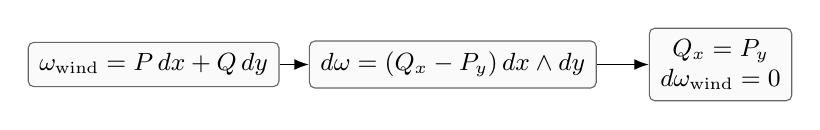
\begin{tikzpicture}[>=Latex, every node/.style={font=\small}]
  \node[smallvisual] (form) at (0,0)
    {$\omega_{\mathrm{wind}}=P\,dx+Q\,dy$};
  \node[smallvisual] (test) at (3.8,0)
    {$d\omega=(Q_x-P_y)\,dx\wedge dy$};
  \node[smallvisual] (zero) at (7.2,0)
    {$Q_x=P_y$\\ \(d\omega_{\mathrm{wind}}=0\)};
  \draw[->, line width=0.5pt] (form) -- (test);
  \draw[->, line width=0.5pt] (test) -- (zero);
\end{tikzpicture}
\end{center}

\textbf{1.2.} With \(x=\cos t\), \(y=\sin t\), one has
\[
  dx=-\sin t\,dt,\qquad dy=\cos t\,dt.
\]
Thus
\[
  -y\,dx+x\,dy=\sin^2t\,dt+\cos^2t\,dt=dt,
\]
and the denominator is \(1\).  The integral from \(0\) to \(2\pi\) is
\(2\pi\).

\begin{center}
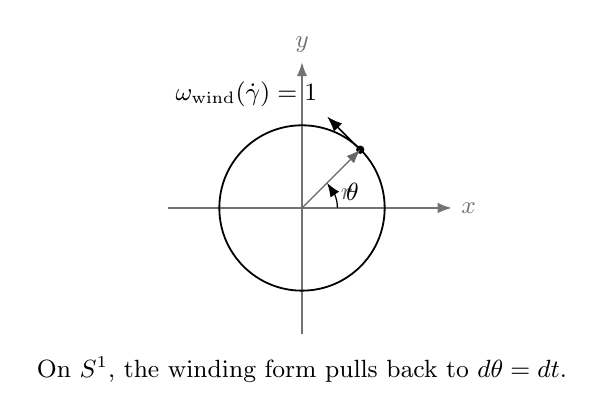
\begin{tikzpicture}[>=Latex, scale=1.0, every node/.style={font=\small}]
  \draw[->, black!55, line width=0.45pt] (-1.7,0) -- (1.9,0) node[right] {$x$};
  \draw[->, black!55, line width=0.45pt] (0,-1.6) -- (0,1.85) node[above] {$y$};
  \draw[black, line width=0.65pt] (0,0) circle (1.05);
  \fill[black] (0.74,0.74) circle (1.5pt);
  \draw[->, line width=0.55pt] (0.74,0.74) -- (0.32,1.16)
    node[above left] {$\omega_{\mathrm{wind}}(\dot\gamma)=1$};
  \draw[->, line width=0.45pt, black!60] (0,0) -- (0.74,0.74)
    node[midway, below right] {$r$};
  \draw[->, line width=0.45pt] (0.45,0)
    arc[start angle=0,end angle=45,radius=0.45];
  \node at (0.64,0.2) {$\theta$};
  \node[align=center] at (0,-2.05)
    {On \(S^1\), the winding form pulls back to \(d\theta=dt\).};
\end{tikzpicture}
\end{center}

\textbf{1.3.} Write \(f=(z-p)^m u(z)\), where \(u(p)\ne0\).  Then
\[
  \frac{df}{f}=m\,\frac{dz}{z-p}+\frac{du}{u}.
\]
The second term is holomorphic near \(p\), so the residue is \(m=\ord_p(f)\).

\begin{center}
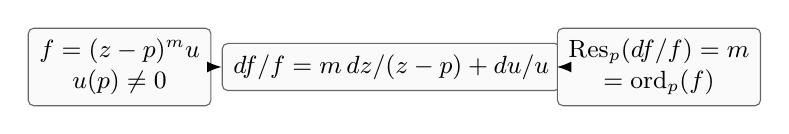
\begin{tikzpicture}[>=Latex, every node/.style={font=\small}]
  \node[smallvisual] (factor) at (0,0)
    {$f=(z-p)^m u$\\ \(u(p)\ne0\)};
  \node[smallvisual] (log) at (3.45,0)
    {$df/f=m\,dz/(z-p)+du/u$};
  \node[smallvisual] (res) at (6.85,0)
    {$\Res_p(df/f)=m$\\ \(=\ord_p(f)\)};
  \draw[->, line width=0.5pt] (factor) -- (log);
  \draw[->, line width=0.5pt] (log) -- (res);
\end{tikzpicture}
\end{center}

\textbf{1.4.} By Exercise 1.3, the residue of \(df/f\) at \(p\) is
\(\ord_p(f)\).  On a compact Riemann surface the sum of residues of a
meromorphic one-form is zero.  Therefore
\[
  0=\sum_p\Res_p(df/f)=\sum_p\ord_p(f)=\degdiv\divisor(f).
\]

\begin{center}
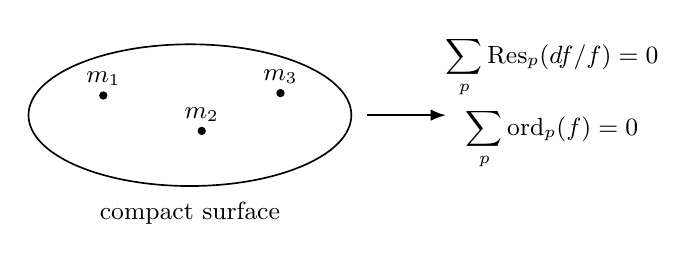
\begin{tikzpicture}[>=Latex, every node/.style={font=\small}]
  \draw[line width=0.6pt] (0,0) ellipse (2.05 and 0.9);
  \foreach \x/\y/\m in {-1.1/0.25/{m_1},0.15/-0.2/{m_2},1.15/0.28/{m_3}}{
    \fill[black] (\x,\y) circle (1.5pt);
    \node[above] at (\x,\y) {$\m$};
  }
  \node[align=center] at (4.6,0.15)
    {$\displaystyle\sum_p\Res_p(df/f)=0$\\[3pt]
     \(\displaystyle\sum_p\ord_p(f)=0\)};
  \draw[->, line width=0.55pt] (2.25,0) -- (3.25,0);
  \node at (0,-1.25) {compact surface};
\end{tikzpicture}
\end{center}

\section{Chapter 2}

\textbf{2.1.} If \(\chi=0\), then \(0=2-2g\), so \(g=1\).

\begin{center}
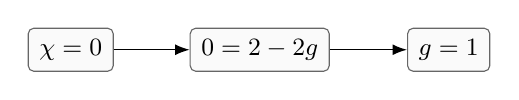
\begin{tikzpicture}[>=Latex, every node/.style={font=\small}]
  \node[smallvisual] (chi) at (0,0) {$\chi=0$};
  \node[smallvisual] (eq) at (2.4,0) {$0=2-2g$};
  \node[smallvisual] (genus) at (4.8,0) {$g=1$};
  \draw[->, line width=0.5pt] (chi) -- (eq);
  \draw[->, line width=0.5pt] (eq) -- (genus);
\end{tikzpicture}
\end{center}

\textbf{2.2.} Noncompact surfaces need not give compact images, so a maximum of
\(|f|\) may not exist.  For example, \(f(z)=z\) on \(\C\) is holomorphic and
nonconstant.

\begin{center}
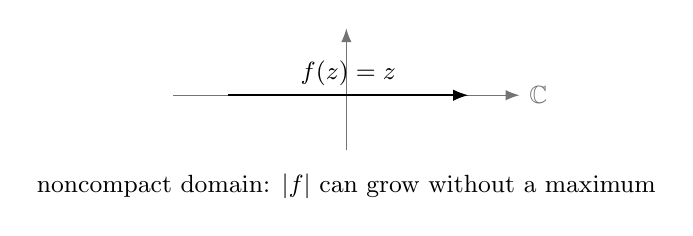
\begin{tikzpicture}[>=Latex, every node/.style={font=\small}]
  \draw[->, black!55, line width=0.45pt] (-2.2,0) -- (2.2,0) node[right] {$\C$};
  \draw[->, black!55, line width=0.45pt] (0,-0.7) -- (0,0.85);
  \draw[->, line width=0.55pt] (-1.5,0) -- (1.55,0)
    node[midway, above] {$f(z)=z$};
  \node[align=center] at (0,-1.15)
    {noncompact domain: \(|f|\) can grow without a maximum};
\end{tikzpicture}
\end{center}

\textbf{2.3.} For a nonzero meromorphic function, zeros and poles are isolated.
An infinite subset of a compact surface has an accumulation point.  That would
contradict isolation: a holomorphic function with accumulating zeros is
identically zero locally, and poles are isolated by the local form
\((z-p)^{-m}u(z)\).  Hence the zero and pole sets are finite.

\begin{center}
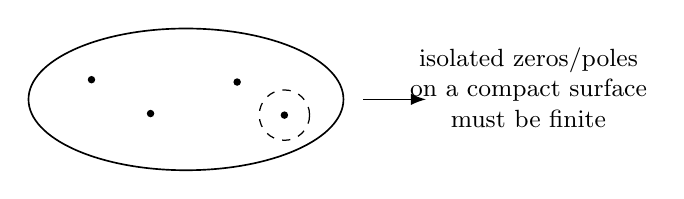
\begin{tikzpicture}[>=Latex, every node/.style={font=\small}]
  \draw[line width=0.6pt] (0,0) ellipse (2.0 and 0.9);
  \foreach \x/\y in {-1.2/0.25,-0.45/-0.18,0.65/0.22,1.25/-0.2}{
    \fill[black] (\x,\y) circle (1.35pt);}
  \draw[dashed, line width=0.45pt] (1.25,-0.2) circle (0.32);
  \node[align=center] at (4.35,0.15)
    {isolated zeros/poles\\on a compact surface\\must be finite};
  \draw[->, line width=0.55pt] (2.25,0) -- (3.05,0);
\end{tikzpicture}
\end{center}

\textbf{2.4.} A parallelogram with opposite sides identified has one face, two
edge classes, and one vertex class.  Hence
\[
  \chi=1-2+1=0.
\]
Since \(\chi=2-2g\), the quotient has \(g=1\).  Thus the quotient surface is a
torus.

\begin{center}
\begin{tikzpicture}[>=Latex, every node/.style={font=\small}]
  \coordinate (A) at (0,0);
  \coordinate (B) at (2.7,0);
  \coordinate (C) at (3.55,1.45);
  \coordinate (D) at (0.85,1.45);
  \draw[line width=0.6pt] (A)--(B)--(C)--(D)--cycle;
  \draw[->, line width=0.55pt] ($(A)!0.36!(B)$) -- ($(A)!0.64!(B)$);
  \draw[->, line width=0.55pt] ($(D)!0.64!(C)$) -- ($(D)!0.36!(C)$);
  \draw[->, line width=0.55pt] ($(A)!0.35!(D)$) -- ($(A)!0.65!(D)$);
  \draw[->, line width=0.55pt] ($(B)!0.65!(C)$) -- ($(B)!0.35!(C)$);
  \node[below] at (1.35,0) {$\omega_1$};
  \node[left] at (0.42,0.72) {$\omega_2$};
  \draw[->, line width=0.55pt] (4.1,0.72) -- node[above] {identify sides} (5.3,0.72);
  \begin{scope}[xshift=6.9cm, yshift=0.72cm, scale=0.23]
    \drawprecisetorus
  \end{scope}
  \node[align=center] at (6.9,-1.0)
    {one face, two edge classes,\\one vertex class};
\end{tikzpicture}
\end{center}

\section{Chapter 3}

\textbf{3.1.} If \(u'=u+\lambda\) and \(v'=v+\mu\), then
\[
  u'+v'=u+v+\lambda+\mu.
\]
Since \(\lambda+\mu\in\Lambda\), this represents the same class as \(u+v\).

\begin{center}
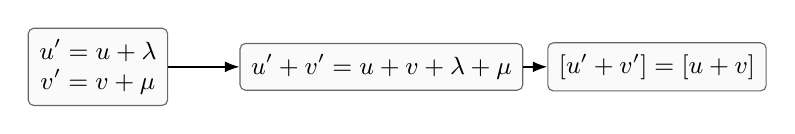
\begin{tikzpicture}[>=Latex, every node/.style={font=\small}]
  \node[smallvisual] (reps) at (0,0)
    {$u'=u+\lambda$\\ \(v'=v+\mu\)};
  \node[smallvisual] (sum) at (3.6,0)
    {$u'+v'=u+v+\lambda+\mu$};
  \node[smallvisual] (same) at (7.1,0)
    {$[u'+v']=[u+v]$};
  \draw[->, line width=0.5pt] (reps) -- (sum);
  \draw[->, line width=0.5pt] (sum) -- (same);
\end{tikzpicture}
\end{center}

\textbf{3.2.} A matrix in \(\GL_2(\Z)\) gives integer combinations of
\(\omega_1,\omega_2\), and its inverse also has integer entries.  Thus each old
basis vector is an integer combination of the new ones and conversely, so the
generated subgroup is unchanged.

\begin{center}
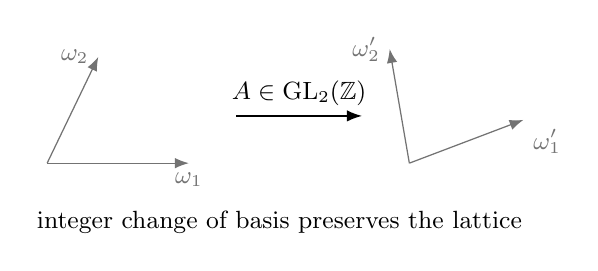
\begin{tikzpicture}[>=Latex, every node/.style={font=\small}]
  \draw[->, black!55, line width=0.45pt] (0,0) -- (1.8,0) node[below] {$\omega_1$};
  \draw[->, black!55, line width=0.45pt] (0,0) -- (0.65,1.35) node[left] {$\omega_2$};
  \draw[->, line width=0.55pt] (2.4,0.6) -- node[above] {$A\in\GL_2(\Z)$} (4.0,0.6);
  \begin{scope}[xshift=4.6cm]
    \draw[->, black!55, line width=0.45pt] (0,0) -- (1.45,0.55) node[below right] {$\omega'_1$};
    \draw[->, black!55, line width=0.45pt] (0,0) -- (-0.25,1.45) node[left] {$\omega'_2$};
  \end{scope}
  \node[align=center] at (2.95,-0.75)
    {integer change of basis preserves the lattice};
\end{tikzpicture}
\end{center}

\textbf{3.3.} The ratio \(\tau=\omega_2/\omega_1\) is non-real because, if
\(\tau\in\R\), then \(\omega_2=\tau\omega_1\) would make
\(\omega_1,\omega_2\) real-linearly dependent.  If \(\tau=a+ib\) with
\(b<0\), swapping the basis vectors gives the new ratio
\[
  \frac{\omega_1}{\omega_2}=\frac1{\tau}
  =\frac{a-ib}{a^2+b^2},
\]
whose imaginary part is \(-b/(a^2+b^2)>0\).  Hence an oriented basis can be
chosen with \(\tau\in\HH\).

\begin{center}
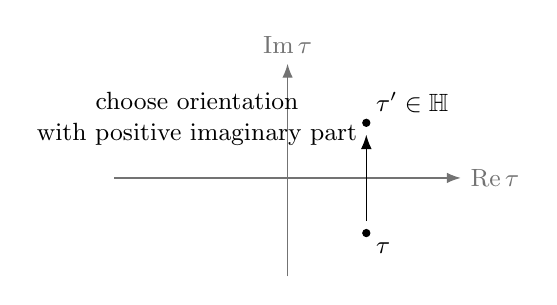
\begin{tikzpicture}[>=Latex, every node/.style={font=\small}]
  \draw[->, black!55, line width=0.45pt] (-2.2,0) -- (2.2,0) node[right] {$\operatorname{Re}\tau$};
  \draw[->, black!55, line width=0.45pt] (0,-1.25) -- (0,1.45) node[above] {$\operatorname{Im}\tau$};
  \fill[black] (1.0,-0.7) circle (1.5pt) node[below right] {$\tau$};
  \fill[black] (1.0,0.7) circle (1.5pt) node[above right] {$\tau'\in\HH$};
  \draw[->, line width=0.5pt] (1.0,-0.55) -- (1.0,0.55);
  \node[align=center] at (-1.15,0.75)
    {choose orientation\\with positive imaginary part};
\end{tikzpicture}
\end{center}

\textbf{3.4.} The map is well-defined because if \(z'=z+\lambda\), then
\[
  z'+a=z+a+\lambda,
\]
so \([z'+a]=[z+a]\).  It is holomorphic because it is induced locally by the
holomorphic map \(z\mapsto z+a\) on \(\C\).  Its inverse is translation by
\(-a\), so it is biholomorphic.

\begin{center}
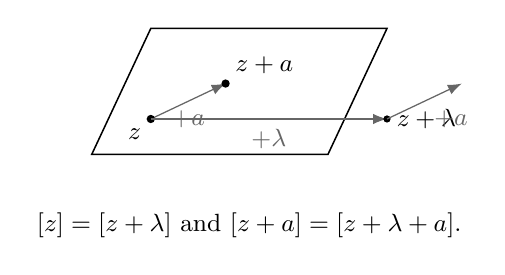
\begin{tikzpicture}[>=Latex, every node/.style={font=\small}]
  \coordinate (A) at (0,0);
  \coordinate (B) at (3.0,0);
  \coordinate (C) at (3.75,1.6);
  \coordinate (D) at (0.75,1.6);
  \draw[line width=0.55pt] (A)--(B)--(C)--(D)--cycle;
  \draw[->, line width=0.45pt, black!60] (0.75,0.45) -- (1.7,0.9)
    node[midway, below] {$+a$};
  \fill[black] (0.75,0.45) circle (1.5pt) node[below left] {$z$};
  \fill[black] (1.7,0.9) circle (1.5pt) node[above right] {$z+a$};
  \draw[->, line width=0.45pt, black!60] (0.75,0.45) -- (3.75,0.45)
    node[midway, below] {$+\lambda$};
  \fill[black] (3.75,0.45) circle (1.3pt) node[right] {$z+\lambda$};
  \draw[->, line width=0.45pt, black!60] (3.75,0.45) -- (4.7,0.9)
    node[midway, below right] {$+a$};
  \node[align=center] at (2,-0.9)
    {\([z]=[z+\lambda]\) and \([z+a]=[z+\lambda+a]\).};
\end{tikzpicture}
\end{center}

\textbf{3.5.} For a map \(F:G\to H\), the checklist is:
\[
\begin{array}{c|c}
\text{condition} & \text{calculation or property}\\ \hline
\text{group homomorphism} & F(x+y)=F(x)+F(y)\\
\text{holomorphic map} & F \text{ is holomorphic in local complex charts}\\
\text{holomorphic inverse} & F^{-1} \text{ exists and is holomorphic.}
\end{array}
\]
Thus an isomorphism of complex Lie groups is simultaneously a biholomorphism and
a group isomorphism, not merely an abstract abelian-group isomorphism.

\begin{center}
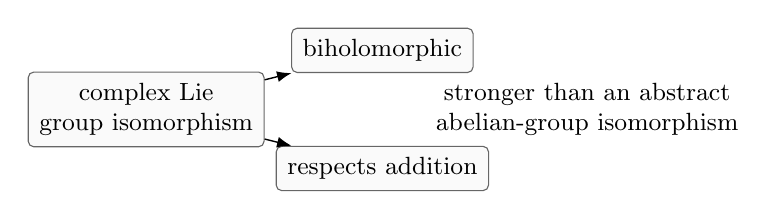
\begin{tikzpicture}[>=Latex, every node/.style={font=\small}]
  \node[smallvisual] (iso) at (0,0) {complex Lie\\group isomorphism};
  \node[smallvisual] (hol) at (3.0,0.75) {biholomorphic};
  \node[smallvisual] (grp) at (3.0,-0.75) {respects addition};
  \draw[->, line width=0.5pt] (iso) -- (hol);
  \draw[->, line width=0.5pt] (iso) -- (grp);
  \node[align=center] at (5.6,0)
    {stronger than an abstract\\abelian-group isomorphism};
\end{tikzpicture}
\end{center}

\section{Chapter 4}

\textbf{4.1.} A nonconstant elliptic function cannot be holomorphic, so it has a
pole.  If the total pole order were \(1\), there would be exactly one simple
pole.  Its Laurent expansion would have a nonzero coefficient of
\((z-a)^{-1}\), hence a nonzero residue.  This contradicts the residue-sum law
for elliptic functions.  Therefore the total pole order is at least \(2\).

\begin{center}
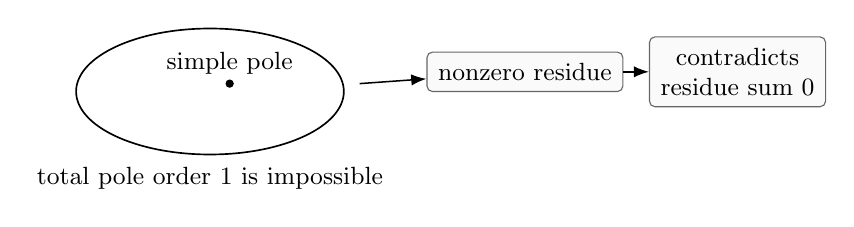
\begin{tikzpicture}[>=Latex, every node/.style={font=\small}]
  \draw[line width=0.6pt] (0,0) ellipse (1.7 and 0.8);
  \fill[black] (0.25,0.1) circle (1.5pt) node[above] {simple pole};
  \node[smallvisual] (res) at (4.0,0.25) {nonzero residue};
  \node[smallvisual] (bad) at (6.7,0.25) {contradicts\\residue sum \(0\)};
  \draw[->, line width=0.55pt] (1.9,0.1) -- (res);
  \draw[->, line width=0.55pt] (res) -- (bad);
  \node at (0,-1.1) {total pole order \(1\) is impossible};
\end{tikzpicture}
\end{center}

\textbf{4.2.} Choose a period parallelogram whose boundary contains no zeros or
poles of \(f\).  Apply the argument principle to \(f\) on its boundary:
\[
  \frac{1}{2\pi i}\int_{\partial P}\frac{f'}{f}\,dz.
\]
Opposite sides cancel by periodicity.  The integral is therefore zero, and it
equals the number of zeros minus the number of poles, counted with
multiplicity.

\begin{center}
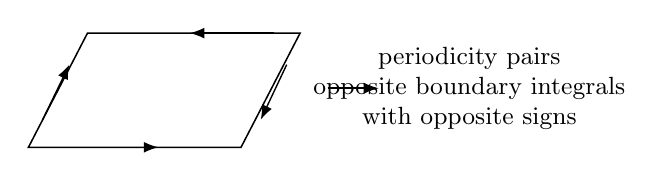
\begin{tikzpicture}[>=Latex, every node/.style={font=\small}]
  \coordinate (A) at (0,0);
  \coordinate (B) at (2.7,0);
  \coordinate (C) at (3.45,1.45);
  \coordinate (D) at (0.75,1.45);
  \draw[line width=0.55pt] (A)--(B)--(C)--(D)--cycle;
  \draw[->, line width=0.5pt] (0.55,0) -- (1.65,0);
  \draw[->, line width=0.5pt] (3.12,1.45) -- (2.05,1.45);
  \draw[->, line width=0.5pt] (0.18,0.35) -- (0.52,1.05);
  \draw[->, line width=0.5pt] (3.28,1.05) -- (2.95,0.35);
  \node[align=center] at (5.6,0.75)
    {periodicity pairs\\opposite boundary integrals\\with opposite signs};
  \draw[->, line width=0.55pt] (3.8,0.75) -- (4.45,0.75);
\end{tikzpicture}
\end{center}

\textbf{4.3.} Changing a lift \(z_i\) by a lattice element changes the weighted
sum by an element of \(\Lambda\).  Therefore the Abel sum is intrinsic only
modulo \(\Lambda\), that is, as a point of \(\C/\Lambda\).

\begin{center}
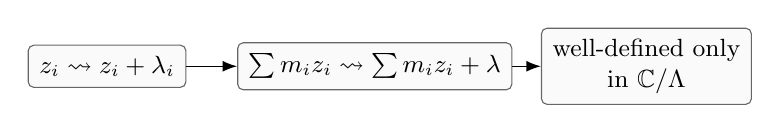
\begin{tikzpicture}[>=Latex, every node/.style={font=\small}]
  \node[smallvisual] (lift) at (0,0)
    {$z_i\rightsquigarrow z_i+\lambda_i$};
  \node[smallvisual] (sum) at (3.4,0)
    {$\sum m_i z_i\rightsquigarrow
      \sum m_i z_i+\lambda$};
  \node[smallvisual] (quot) at (6.85,0)
    {well-defined only\\in \(\C/\Lambda\)};
  \draw[->, line width=0.5pt] (lift) -- (sum);
  \draw[->, line width=0.5pt] (sum) -- (quot);
\end{tikzpicture}
\end{center}

\textbf{4.4.} If \(F\) is meromorphic on \(T\), then \(F\circ q\) is meromorphic
on \(\C\) and satisfies
\[
  F(q(z+\lambda))=F(q(z))
\]
for all \(\lambda\in\Lambda\).  Conversely, if \(f\) is elliptic, define
\(F([z])=f(z)\).  Periodicity makes this well-defined, and the quotient charts
show that \(F\) is meromorphic on \(T\).

\begin{center}
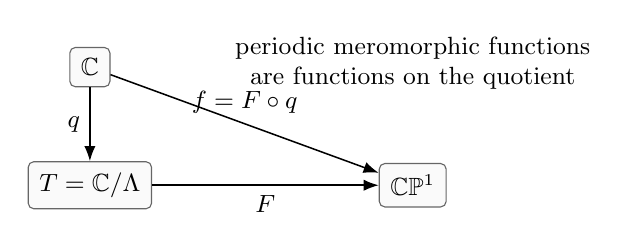
\begin{tikzpicture}[>=Latex, every node/.style={font=\small}]
  \node[smallvisual] (C) at (0,0.75) {$\C$};
  \node[smallvisual] (T) at (0,-0.75) {$T=\C/\Lambda$};
  \node[smallvisual] (vals) at (4.1,-0.75) {$\CP^1$};
  \draw[->, line width=0.55pt] (C) -- node[left] {$q$} (T);
  \draw[->, line width=0.55pt] (T) -- node[below] {$F$} (vals);
  \draw[->, line width=0.55pt] (C) -- node[above] {$f=F\circ q$} (vals);
  \node[align=center] at (4.1,0.8)
    {periodic meromorphic functions\\are functions on the quotient};
\end{tikzpicture}
\end{center}

\textbf{4.5.} For
\[
  \divisor(f)=[a_1]+[a_2]-[b_1]-[b_2],
\]
the third Liouville law gives
\[
  a_1+a_2-b_1-b_2\in\Lambda.
\]
Modulo \(\Lambda\), this is
\[
  a_1+a_2-b_1-b_2\equiv0\pmod{\Lambda}.
\]
By the definition of the Abel-sum map, this says
\[
  \smap(\divisor(f))=0\in T.
\]

\begin{center}
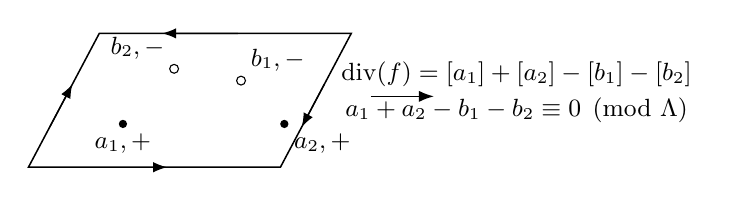
\begin{tikzpicture}[>=Latex, every node/.style={font=\small}]
  \coordinate (A) at (0,0);
  \coordinate (B) at (3.2,0);
  \coordinate (C) at (4.1,1.7);
  \coordinate (D) at (0.9,1.7);
  \draw[line width=0.55pt] (A)--(B)--(C)--(D)--cycle;
  \draw[->, line width=0.45pt] ($(A)!0.25!(B)$) -- ($(A)!0.55!(B)$);
  \draw[->, line width=0.45pt] ($(D)!0.55!(C)$) -- ($(D)!0.25!(C)$);
  \draw[->, line width=0.45pt] ($(A)!0.3!(D)$) -- ($(A)!0.62!(D)$);
  \draw[->, line width=0.45pt] ($(B)!0.62!(C)$) -- ($(B)!0.3!(C)$);
  \fill[black] (1.2,0.55) circle (1.5pt) node[below] {$a_1,+$};
  \fill[white] (2.7,1.1) circle (1.6pt);
  \draw[black] (2.7,1.1) circle (1.6pt) node[above right] {$b_1,-$};
  \fill[black] (3.25,0.55) circle (1.5pt) node[below right] {$a_2,+$};
  \fill[white] (1.85,1.25) circle (1.6pt);
  \draw[black] (1.85,1.25) circle (1.6pt) node[above left] {$b_2,-$};
  \node[align=center] at (6.2,0.95)
    {$\divisor(f)=[a_1]+[a_2]-[b_1]-[b_2]$\\[2pt]
     \(a_1+a_2-b_1-b_2\equiv0\pmod{\Lambda}\)};
  \draw[->, line width=0.55pt] (4.35,0.9) -- (5.15,0.9);
\end{tikzpicture}
\end{center}

\section{Chapter 5}

\textbf{5.1.} Replacing \(z\) by \(-z\) permutes the lattice terms
\(\lambda\mapsto-\lambda\) and leaves the series unchanged.  Hence
\(\wp(-z)=\wp(z)\).

\begin{center}
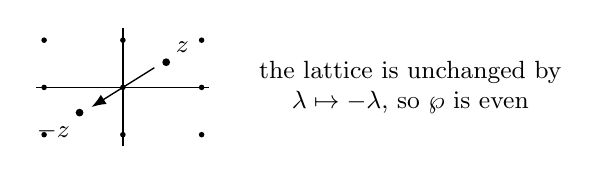
\begin{tikzpicture}[>=Latex, every node/.style={font=\small}]
  \draw[line width=0.5pt] (-1.1,0) -- (1.1,0);
  \draw[line width=0.5pt] (0,-0.75) -- (0,0.75);
  \foreach \x in {-1,0,1}{\foreach \y in {-0.6,0,0.6}{\fill[black] (\x,\y) circle (1pt);}}
  \fill[black] (0.55,0.32) circle (1.4pt) node[above right] {$z$};
  \fill[black] (-0.55,-0.32) circle (1.4pt) node[below left] {$-z$};
  \draw[->, line width=0.5pt] (0.4,0.25) -- (-0.4,-0.25);
  \node[align=center] at (3.65,0)
    {the lattice is unchanged by\\\(\lambda\mapsto-\lambda\), so \(\wp\) is even};
\end{tikzpicture}
\end{center}

\textbf{5.2.} The derivative of an even function is odd: differentiating
\(\wp(-z)=\wp(z)\) gives \(-\wp'(-z)=\wp'(z)\), so
\(\wp'(-z)=-\wp'(z)\).

\begin{center}
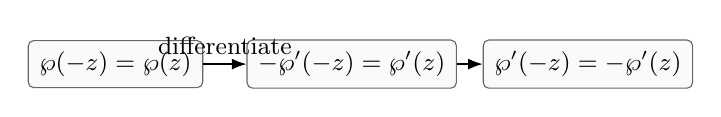
\begin{tikzpicture}[>=Latex, every node/.style={font=\small}]
  \node[smallvisual] (even) at (0,0) {$\wp(-z)=\wp(z)$};
  \node[smallvisual] (diff) at (3.0,0) {$-\wp'(-z)=\wp'(z)$};
  \node[smallvisual] (odd) at (6.0,0) {$\wp'(-z)=-\wp'(z)$};
  \draw[->, line width=0.5pt] (even) -- node[above] {differentiate} (diff);
  \draw[->, line width=0.5pt] (diff) -- (odd);
\end{tikzpicture}
\end{center}

\textbf{5.3.} The equation
\[
  \wp'^2=4\wp^3-g_2\wp-g_3
\]
is a polynomial equation for \(\wp'\) with coefficients in \(\C(\wp)\).  It is
quadratic in \(\wp'\), so \(\wp'\) has degree at most \(2\) over \(\C(\wp)\).

\begin{center}
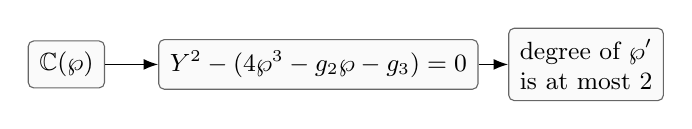
\begin{tikzpicture}[>=Latex, every node/.style={font=\small}]
  \node[smallvisual] (field) at (0,0) {$\C(\wp)$};
  \node[smallvisual] (quad) at (3.2,0)
    {$Y^2-(4\wp^3-g_2\wp-g_3)=0$};
  \node[smallvisual] (deg) at (6.6,0)
    {degree of \(\wp'\)\\is at most \(2\)};
  \draw[->, line width=0.5pt] (field) -- (quad);
  \draw[->, line width=0.5pt] (quad) -- (deg);
\end{tikzpicture}
\end{center}

\textbf{5.4.} From the Laurent expansion
\[
  \wp(z)=z^{-2}+O(z^2),
\]
\(\wp\) has a pole of order \(2\) at \(O\).  From
\[
  \wp'(z)=-2z^{-3}+O(z),
\]
\(\wp'\) has a pole of order \(3\) at \(O\).

\begin{center}
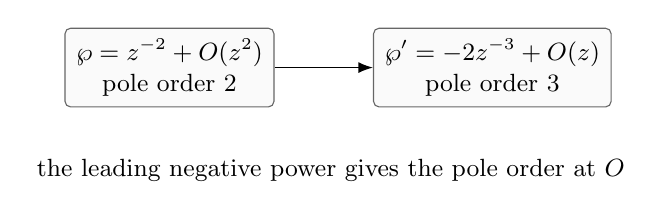
\begin{tikzpicture}[>=Latex, every node/.style={font=\small}]
  \node[smallvisual] (wp) at (0,0.55)
    {$\wp=z^{-2}+O(z^2)$\\ pole order \(2\)};
  \node[smallvisual] (wpp) at (4.1,0.55)
    {$\wp'=-2z^{-3}+O(z)$\\ pole order \(3\)};
  \node[align=center] at (2.05,-0.75)
    {the leading negative power gives the pole order at \(O\)};
  \draw[->, line width=0.5pt] (wp) -- (wpp);
\end{tikzpicture}
\end{center}

\textbf{5.5.} Substituting \(x=\wp(z)\) and \(y=\wp'(z)\) into the differential
equation gives
\[
  y^2=4x^3-g_2x-g_3.
\]
Thus every point \((\wp(z),\wp'(z))\), away from the pole, lies on the affine
cubic.

\begin{center}
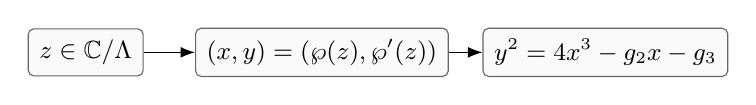
\begin{tikzpicture}[>=Latex, every node/.style={font=\small}]
  \node[smallvisual] (torus) at (0,0) {$z\in\C/\Lambda$};
  \node[smallvisual] (coord) at (3.0,0) {$(x,y)=(\wp(z),\wp'(z))$};
  \node[smallvisual] (curve) at (6.6,0) {$y^2=4x^3-g_2x-g_3$};
  \draw[->, line width=0.5pt] (torus) -- (coord);
  \draw[->, line width=0.5pt] (coord) -- (curve);
\end{tikzpicture}
\end{center}

\section{Chapter 6}

\textbf{6.1.} The function \(z^2(z-1)^{-3}\) has a zero of order \(2\) at
\(0\), a pole of order \(3\) at \(1\), and a pole/zero contribution at
\(\infty\) chosen so the total degree is zero.  In the coordinate \(w=1/z\),
the function is
\[
  \frac{w}{(1-w)^3},
\]
so it has a zero of order \(1\) at \(\infty\).  Hence
\[
  \divisor(z^2(z-1)^{-3})=2[0]-3[1]+[\infty].
\]

\begin{center}
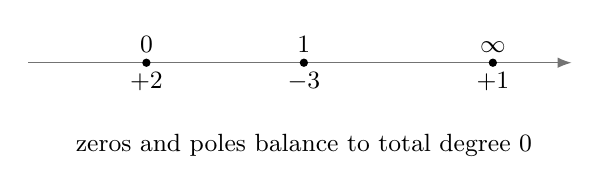
\begin{tikzpicture}[>=Latex, every node/.style={font=\small}]
  \draw[->, black!55, line width=0.45pt] (-0.5,0) -- (6.4,0);
  \foreach \x/\lab/\mult in {1/{0}/{+2},3/{1}/{-3},5.4/{\infty}/{+1}}{
    \fill[black] (\x,0) circle (1.5pt);
    \node[above] at (\x,0) {$\lab$};
    \node[below] at (\x,0) {$\mult$};
  }
  \node[align=center] at (3,-1.05)
    {zeros and poles balance to total degree \(0\)};
\end{tikzpicture}
\end{center}

\textbf{6.2.} Products of meromorphic functions add divisors:
\[
  \divisor(fg)=\divisor(f)+\divisor(g).
\]
Inverses negate divisors, and constants give the zero divisor.  Since principal
divisors have degree zero, \(\Prin(X)\) is a subgroup of \(\Div^0(X)\).

\begin{center}
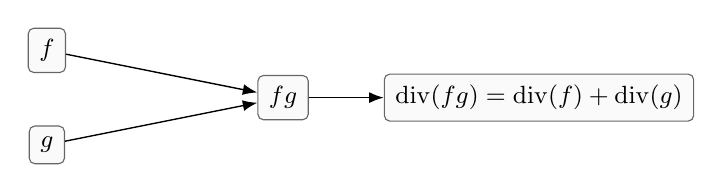
\begin{tikzpicture}[>=Latex, every node/.style={font=\small}]
  \node[smallvisual] (f) at (0,0.6) {$f$};
  \node[smallvisual] (g) at (0,-0.6) {$g$};
  \node[smallvisual] (fg) at (3.0,0) {$fg$};
  \node[smallvisual] (div) at (6.25,0)
    {$\divisor(fg)=\divisor(f)+\divisor(g)$};
  \draw[->, line width=0.5pt] (f) -- (fg);
  \draw[->, line width=0.5pt] (g) -- (fg);
  \draw[->, line width=0.5pt] (fg) -- (div);
\end{tikzpicture}
\end{center}

\textbf{6.3.} The coefficients of \([P]-[O]\) are \(1\) and \(-1\), so the
degree is \(1-1=0\).

\begin{center}
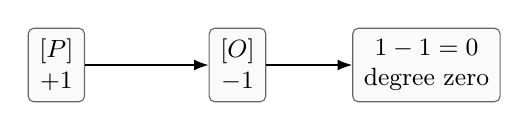
\begin{tikzpicture}[>=Latex, every node/.style={font=\small}]
  \node[smallvisual] (P) at (0,0) {$[P]$\\ \(+1\)};
  \node[smallvisual] (O) at (2.3,0) {$[O]$\\ \(-1\)};
  \node[smallvisual] (zero) at (4.7,0) {$1-1=0$\\ degree zero};
  \draw[->, line width=0.5pt] (P) -- (O);
  \draw[->, line width=0.5pt] (O) -- (zero);
\end{tikzpicture}
\end{center}

\textbf{6.4.} The divisor
\[
  [P]+[Q]-2[O]
\]
has degree \(1+1-2=0\).  Therefore it lies in \(\Div^0(X)\), and its class
modulo principal divisors is an element of \(\Pic^0(X)\).

\begin{center}
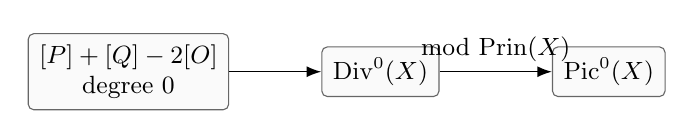
\begin{tikzpicture}[>=Latex, every node/.style={font=\small}]
  \node[smallvisual] (div) at (0,0)
    {$[P]+[Q]-2[O]$\\ degree \(0\)};
  \node[smallvisual] (Div0) at (3.2,0) {$\Div^0(X)$};
  \node[smallvisual] (Pic) at (6.1,0) {$\Pic^0(X)$};
  \draw[->, line width=0.5pt] (div) -- (Div0);
  \draw[->, line width=0.5pt] (Div0) -- node[above] {mod \(\Prin(X)\)} (Pic);
\end{tikzpicture}
\end{center}

\textbf{6.5.} Two degree-zero divisors \(D,D'\) define the same element of
\(\Pic^0(X)=\Div^0(X)/\Prin(X)\) exactly when
\[
  D-D'\in\Prin(X).
\]
This is the defining equivalence relation in the quotient group.

\begin{center}
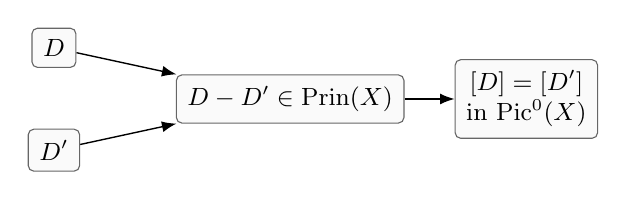
\begin{tikzpicture}[>=Latex, every node/.style={font=\small}]
  \node[smallvisual] (D) at (0,0.65) {$D$};
  \node[smallvisual] (Dp) at (0,-0.65) {$D'$};
  \node[smallvisual] (diff) at (3.0,0) {$D-D'\in\Prin(X)$};
  \node[smallvisual] (same) at (6.0,0) {$[D]=[D']$\\in \(\Pic^0(X)\)};
  \draw[->, line width=0.5pt] (D) -- (diff);
  \draw[->, line width=0.5pt] (Dp) -- (diff);
  \draw[->, line width=0.5pt] (diff) -- (same);
\end{tikzpicture}
\end{center}

\section{Chapter 7}

\textbf{7.1.} The dimensions are
\[
  \ell(O)=1,\qquad \ell(2O)=2,\qquad \ell(3O)=3.
\]

\begin{center}
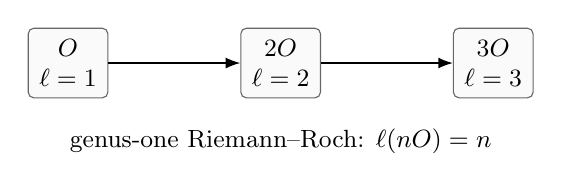
\begin{tikzpicture}[>=Latex, every node/.style={font=\small}]
  \node[smallvisual] (one) at (0,0) {$O$\\ \(\ell=1\)};
  \node[smallvisual] (two) at (2.7,0) {$2O$\\ \(\ell=2\)};
  \node[smallvisual] (three) at (5.4,0) {$3O$\\ \(\ell=3\)};
  \draw[->, line width=0.5pt] (one) -- (two);
  \draw[->, line width=0.5pt] (two) -- (three);
  \node[align=center] at (2.7,-1.0)
    {genus-one Riemann--Roch: \(\ell(nO)=n\)};
\end{tikzpicture}
\end{center}

\textbf{7.2.} A function in \(L(O)\) has at most a simple pole at \(O\) and no
other poles.  If it has no pole, it is holomorphic on the compact torus and is
constant.  If it has a simple pole at \(O\), it has total pole order \(1\),
which is impossible by Exercise 4.1.  Hence every element of \(L(O)\) is
constant.

\begin{center}
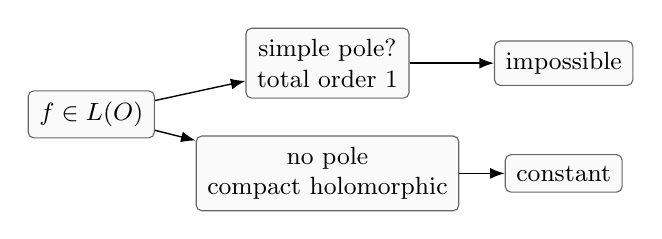
\begin{tikzpicture}[>=Latex, every node/.style={font=\small}]
  \node[smallvisual] (LO) at (0,0) {$f\in L(O)$};
  \node[smallvisual] (simple) at (3.0,0.65) {simple pole?\\total order \(1\)};
  \node[smallvisual] (no) at (6.0,0.65) {impossible};
  \node[smallvisual] (const) at (3.0,-0.75) {no pole\\compact holomorphic};
  \node[smallvisual] (C) at (6.0,-0.75) {constant};
  \draw[->, line width=0.5pt] (LO) -- (simple);
  \draw[->, line width=0.5pt] (simple) -- (no);
  \draw[->, line width=0.5pt] (LO) -- (const);
  \draw[->, line width=0.5pt] (const) -- (C);
\end{tikzpicture}
\end{center}

\textbf{7.3.} The pole orders at \(O\) are \(0,2,3\) for \(1,\wp,\wp'\).  In a
linear relation, the term with the largest pole order cannot be cancelled by
terms with smaller pole order.  Descending through the possible largest pole
orders forces all coefficients to be zero.

\begin{center}
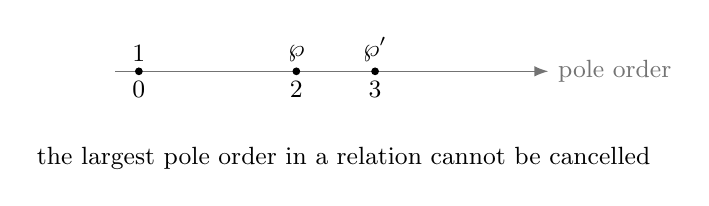
\begin{tikzpicture}[>=Latex, every node/.style={font=\small}]
  \draw[->, black!55, line width=0.45pt] (-0.3,0) -- (5.2,0) node[right] {pole order};
  \foreach \x/\lab in {0/{1},2/{\wp},3/{\wp'}}{
    \fill[black] (\x,0) circle (1.4pt);
    \node[above] at (\x,0) {$\lab$};
    \node[below] at (\x,0) {$\x$};
  }
  \node[align=center] at (2.6,-1.1)
    {the largest pole order in a relation cannot be cancelled};
\end{tikzpicture}
\end{center}

\textbf{7.4.} The constant function satisfies
\[
  \divisor(1)+2[O]=2[O]\ge0,
\]
so \(1\in L(2O)\).  Since \(\wp\) has no poles away from \(O\) and has pole
order \(2\) at \(O\),
\[
  \divisor(\wp)+2[O]\ge0,
\]
so \(\wp\in L(2O)\).  The pole orders \(0\) and \(2\) make \(1,\wp\) linearly
independent.  Since \(\ell(2O)=2\), they form a basis:
\[
  L(2O)=\Span_\C(1,\wp).
\]

\begin{center}
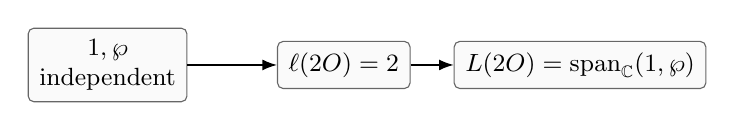
\begin{tikzpicture}[>=Latex, every node/.style={font=\small}]
  \node[smallvisual] (ind) at (0,0) {$1,\wp$\\independent};
  \node[smallvisual] (dim) at (3.0,0) {$\ell(2O)=2$};
  \node[smallvisual] (basis) at (6.0,0) {$L(2O)=\Span_\C(1,\wp)$};
  \draw[->, line width=0.5pt] (ind) -- (dim);
  \draw[->, line width=0.5pt] (dim) -- (basis);
\end{tikzpicture}
\end{center}

\textbf{7.5.} Membership is checked by the divisor inequalities
\[
  \divisor(1)+3[O]=3[O]\ge0,\qquad
  \divisor(\wp)+3[O]\ge0,\qquad
  \divisor(\wp')+3[O]\ge0.
\]
The second inequality holds because \(\wp\) has pole order \(2\le3\) at \(O\);
the third holds because \(\wp'\) has pole order exactly \(3\) at \(O\).  The
functions \(1,\wp,\wp'\) are linearly independent by pole orders \(0,2,3\).
Since \(\ell(3O)=3\), they form a basis:
\[
  L(3O)=\Span_\C(1,\wp,\wp').
\]

\begin{center}
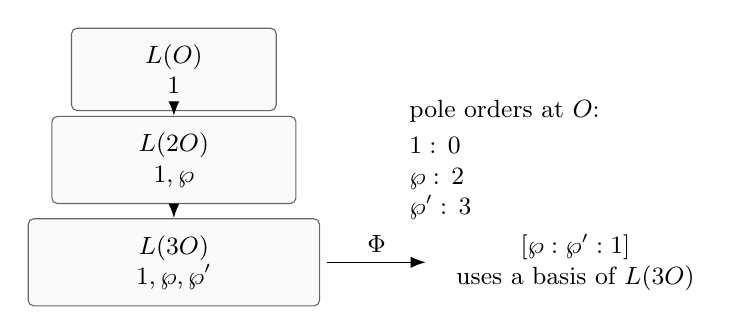
\begin{tikzpicture}[>=Latex, every node/.style={font=\small}]
  \node[visualnode, minimum width=2.6cm] (LO) at (0,1.7) {$L(O)$\\ \(1\)};
  \node[visualnode, minimum width=3.1cm] (L2) at (0,0.55) {$L(2O)$\\ \(1,\wp\)};
  \node[visualnode, minimum width=3.7cm] (L3) at (0,-0.75) {$L(3O)$\\ \(1,\wp,\wp'\)};
  \draw[->, line width=0.5pt] (LO) -- (L2);
  \draw[->, line width=0.5pt] (L2) -- (L3);
  \node[align=left] at (4.2,0.55)
    {pole orders at \(O\):\\[2pt]
     \(1:\,0\)\\
     \(\wp:\,2\)\\
     \(\wp':\,3\)};
  \draw[->, line width=0.55pt] (1.95,-0.75) -- node[above] {\(\Phi\)} (3.2,-0.75);
  \node[align=center] at (5.1,-0.75)
    {\([\wp:\wp':1]\)\\uses a basis of \(L(3O)\)};
\end{tikzpicture}
\end{center}

\section{Chapter 8}

\textbf{8.1.} Choose lifts \(p,q\in\C\) of \(P,Q\).  Then
\[
  \smap([P]-[Q])=p-q\pmod{\Lambda}.
\]
This is exactly the class \(P-Q\) in the quotient group \(T=\C/\Lambda\).

\begin{center}
\begin{tikzpicture}[>=Latex, every node/.style={font=\small}]
  \begin{scope}[scale=0.3]
    \drawprecisetorus
  \end{scope}
  \fill[black] (0.65,0.35) circle (1.5pt) node[above right] {$P$};
  \fill[black] (-0.55,-0.25) circle (1.5pt) node[below left] {$Q$};
  \draw[->, line width=0.5pt] (-0.55,-0.25) -- (0.65,0.35)
    node[midway, above] {$P-Q$};
  \node[align=center] at (3.9,0)
    {\([P]-[Q]\) has Abel sum \(P-Q\) in \(T\)};
\end{tikzpicture}
\end{center}

\textbf{8.2.} Choose lifts \(p,q,0\in\C\) of \(P,Q,O\).  The Abel sum is
\[
  p+q-2\cdot0\equiv p+q\pmod{\Lambda}.
\]
By Abel's theorem, \([P]+[Q]-2[O]\) is principal exactly when this class is
zero, namely when \(p+q\equiv0\pmod{\Lambda}\), or \(P+Q=O\) in \(T\).

\begin{center}
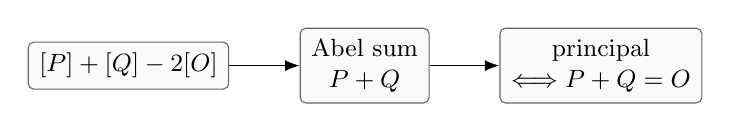
\begin{tikzpicture}[>=Latex, every node/.style={font=\small}]
  \node[smallvisual] (div) at (0,0)
    {$[P]+[Q]-2[O]$};
  \node[smallvisual] (sum) at (3.0,0)
    {Abel sum\\ \(P+Q\)};
  \node[smallvisual] (prin) at (6.0,0)
    {principal\\\(\Longleftrightarrow P+Q=O\)};
  \draw[->, line width=0.5pt] (div) -- (sum);
  \draw[->, line width=0.5pt] (sum) -- (prin);
\end{tikzpicture}
\end{center}

\textbf{8.3.} If \([P]-[O]=[Q]-[O]\), then \([P]-[Q]\) is principal.  Abel's
theorem gives \(P-Q=0\) in \(T\), hence \(P=Q\).

\begin{center}
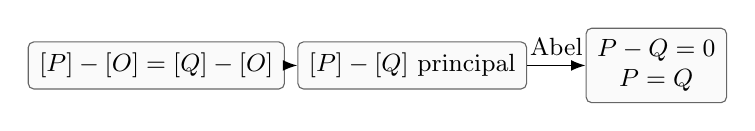
\begin{tikzpicture}[>=Latex, every node/.style={font=\small}]
  \node[smallvisual] (classes) at (0,0)
    {$[P]-[O]=[Q]-[O]$};
  \node[smallvisual] (principal) at (3.25,0)
    {$[P]-[Q]$ principal};
  \node[smallvisual] (same) at (6.35,0)
    {$P-Q=0$\\ \(P=Q\)};
  \draw[->, line width=0.5pt] (classes) -- (principal);
  \draw[->, line width=0.5pt] (principal) -- node[above] {Abel} (same);
\end{tikzpicture}
\end{center}

\textbf{8.4.} Write \(D=\sum_i n_i[p_i]\) and \(D'=\sum_j m_j[q_j]\).  Then
\[
  \smap(D+D')=\sum_i n_i p_i+\sum_j m_j q_j
  =\smap(D)+\smap(D')
\]
in \(\C/\Lambda\).

\begin{center}
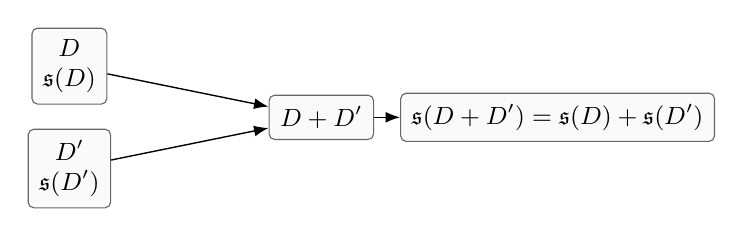
\begin{tikzpicture}[>=Latex, every node/.style={font=\small}]
  \node[smallvisual] (D) at (0,0.65) {$D$\\ \(\smap(D)\)};
  \node[smallvisual] (Dp) at (0,-0.65) {$D'$\\ \(\smap(D')\)};
  \node[smallvisual] (sum) at (3.2,0) {$D+D'$};
  \node[smallvisual] (image) at (6.2,0)
    {$\smap(D+D')=\smap(D)+\smap(D')$};
  \draw[->, line width=0.5pt] (D) -- (sum);
  \draw[->, line width=0.5pt] (Dp) -- (sum);
  \draw[->, line width=0.5pt] (sum) -- (image);
\end{tikzpicture}
\end{center}

\textbf{8.5.} If \(D\) is replaced by \(D+\divisor(f)\), then
\[
  \smap(D+\divisor(f))-\smap(D)=\smap(\divisor(f)).
\]
The divisor \(\divisor(f)\) is principal, so Abel's theorem gives
\(\smap(\divisor(f))=0\).  Therefore \(\smap\) is well-defined on divisor
classes in \(\Pic^0(T)\).  Exercise 8.4 gives additivity, so the induced map is
a group homomorphism.

\begin{center}
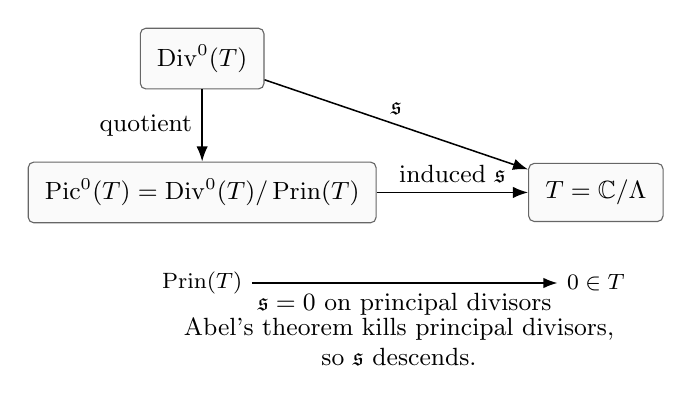
\begin{tikzpicture}[>=Latex, every node/.style={font=\small}]
  \node[visualnode] (Div) at (0,1.15) {$\Div^0(T)$};
  \node[visualnode] (Pic) at (0,-0.55) {$\Pic^0(T)=\Div^0(T)/\Prin(T)$};
  \node[visualnode] (T) at (5.0,-0.55) {$T=\C/\Lambda$};
  \node[font=\footnotesize] (Prin) at (0,-1.7) {$\Prin(T)$};
  \node[font=\footnotesize] (zero) at (5.0,-1.7) {$0\in T$};
  \draw[->, line width=0.55pt] (Div) -- node[left] {quotient} (Pic);
  \draw[->, line width=0.55pt] (Div) -- node[above] {\(\smap\)} (T);
  \draw[->, line width=0.55pt] (Pic) -- node[above] {induced \(\smap\)} (T);
  \draw[->, line width=0.45pt] (Prin) -- node[below] {\(\smap=0\) on principal divisors} (zero);
  \node[align=center] at (2.5,-2.45)
    {Abel's theorem kills principal divisors,\\so \(\smap\) descends.};
\end{tikzpicture}
\end{center}

\section{Chapter 9}

\textbf{9.1.} Homogeneous coordinates may be multiplied by \(z^3\):
\[
  [\wp:\wp':1]=[z+O(z^5):-2+O(z^4):z^3],
\]
which tends to \([0:1:0]\).

\begin{center}
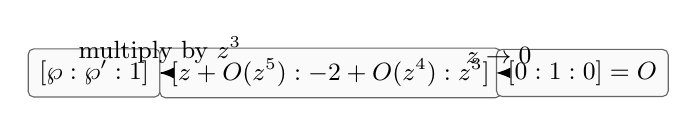
\begin{tikzpicture}[>=Latex, every node/.style={font=\small}]
  \node[smallvisual] (aff) at (0,0)
    {$[\wp:\wp':1]$};
  \node[smallvisual] (scaled) at (3.0,0)
    {$[z+O(z^5):-2+O(z^4):z^3]$};
  \node[smallvisual] (limit) at (6.2,0)
    {$[0:1:0]=O$};
  \draw[->, line width=0.5pt] (aff) -- node[above] {multiply by \(z^3\)} (scaled);
  \draw[->, line width=0.5pt] (scaled) -- node[above] {\(z\to0\)} (limit);
\end{tikzpicture}
\end{center}

\textbf{9.2.} With \(x(z)=\wp(z)\) and \(y(z)=\wp'(z)\),
\[
  x(-z)=\wp(-z)=\wp(z)=x(z),
\]
while
\[
  y(-z)=\wp'(-z)=-\wp'(z)=-y(z).
\]
Thus \(z\mapsto -z\) fixes the \(x\)-coordinate and changes the sign of the
\(y\)-coordinate.

\begin{center}
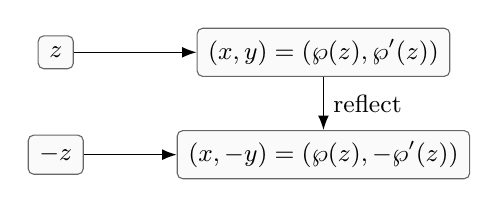
\begin{tikzpicture}[>=Latex, every node/.style={font=\small}]
  \node[smallvisual] (z) at (0,0.65) {$z$};
  \node[smallvisual] (mz) at (0,-0.65) {$-z$};
  \node[smallvisual] (P) at (3.4,0.65) {$(x,y)=(\wp(z),\wp'(z))$};
  \node[smallvisual] (mP) at (3.4,-0.65) {$(x,-y)=(\wp(z),-\wp'(z))$};
  \draw[->, line width=0.5pt] (z) -- (P);
  \draw[->, line width=0.5pt] (mz) -- (mP);
  \draw[->, line width=0.5pt] (P) -- node[right] {reflect} (mP);
\end{tikzpicture}
\end{center}

\textbf{9.3.} For \(F(x,y)=y^2-(4x^3-g_2x-g_3)\), a singular affine point must
satisfy \(F=0\), \(F_y=2y=0\), and \(F_x=-12x^2+g_2=0\).  Thus \(y=0\) and
\(x\) is a repeated root of \(4x^3-g_2x-g_3\).  Conversely, a repeated root gives
such a singular point.

\begin{center}
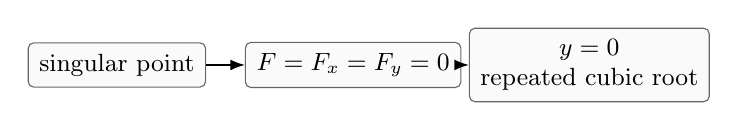
\begin{tikzpicture}[>=Latex, every node/.style={font=\small}]
  \node[smallvisual] (sing) at (0,0) {singular point};
  \node[smallvisual] (partials) at (3.0,0)
    {$F=F_x=F_y=0$};
  \node[smallvisual] (root) at (6.0,0)
    {$y=0$\\ repeated cubic root};
  \draw[->, line width=0.5pt] (sing) -- (partials);
  \draw[->, line width=0.5pt] (partials) -- (root);
\end{tikzpicture}
\end{center}

\textbf{9.4.} Since \(\wp(-z)=\wp(z)\) and \(\wp'(-z)=-\wp'(z)\),
\[
  \Phi(-z)=[\wp(z):-\wp'(z):1]=\ominus\Phi(z).
\]
At \(O\), both sides are \(O=[0:1:0]\).

\begin{center}
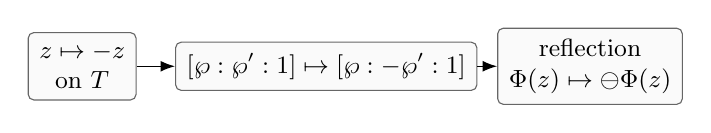
\begin{tikzpicture}[>=Latex, every node/.style={font=\small}]
  \node[smallvisual] (torus) at (0,0) {$z\mapsto -z$\\on \(T\)};
  \node[smallvisual] (coords) at (3.1,0)
    {$[\wp:\wp':1]\mapsto[\wp:-\wp':1]$};
  \node[smallvisual] (cubic) at (6.45,0) {reflection\\\(\Phi(z)\mapsto\ominus\Phi(z)\)};
  \draw[->, line width=0.5pt] (torus) -- (coords);
  \draw[->, line width=0.5pt] (coords) -- (cubic);
\end{tikzpicture}
\end{center}

\textbf{9.5.} The torus notation is \(z\in T\).  The cubic notation is
\(\Phi(z)\in E(\C)\).  The divisor-class notation is
\[
  [\Phi(z)]-[O]\in\Pic^0(E).
\]
The first identification is the Weierstrass map \(\Phi\), and the second is the
Abel-Jacobi divisor-class map \(P\mapsto[P]-[O]\).

\begin{center}
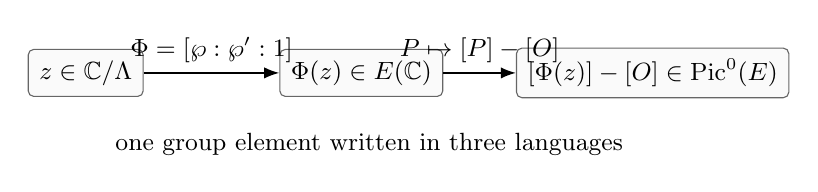
\begin{tikzpicture}[>=Latex, every node/.style={font=\small}]
  \node[smallvisual] (T) at (0,0)
    {$z\in\C/\Lambda$};
  \node[smallvisual] (E) at (3.5,0)
    {$\Phi(z)\in E(\C)$};
  \node[smallvisual] (J) at (7.2,0)
    {$[\Phi(z)]-[O]\in\Pic^0(E)$};
  \draw[->, line width=0.55pt] (T) -- node[above] {\(\Phi=[\wp:\wp':1]\)} (E);
  \draw[->, line width=0.55pt] (E) --
    node[above] {$P\mapsto[P]-[O]$} (J);
  \node[align=center] at (3.6,-0.9)
    {one group element written in three languages};
\end{tikzpicture}
\end{center}

\textbf{9.6.} If \(\Phi(z)=\Phi(w)\) in the affine chart, then equality of
projective coordinates gives
\[
  \wp(z)=\wp(w),\qquad \wp'(z)=\wp'(w).
\]
For a generic \(x\)-value, the equation \(\wp(t)=\wp(z)\) has the two solutions
\[
  t\equiv z,\qquad t\equiv -z \pmod{\Lambda}.
\]
If \(w\equiv -z\), then oddness gives
\[
  \wp'(w)=\wp'(-z)=-\wp'(z).
\]
Together with \(\wp'(w)=\wp'(z)\), this forces \(\wp'(z)=0\).  Thus away from
the branch points where \(\wp'(z)=0\), the second coordinate removes the
generic \(z\) versus \(-z\) ambiguity and gives \(w\equiv z\).  The exceptional
half-period cases, where \(z\equiv -z\) modulo \(\Lambda\), and the point
\(O\) at infinity are handled by the full Weierstrass embedding theorem.  This
calculation is an injectivity check in the generic case, not a complete proof of
the theorem.

\begin{center}
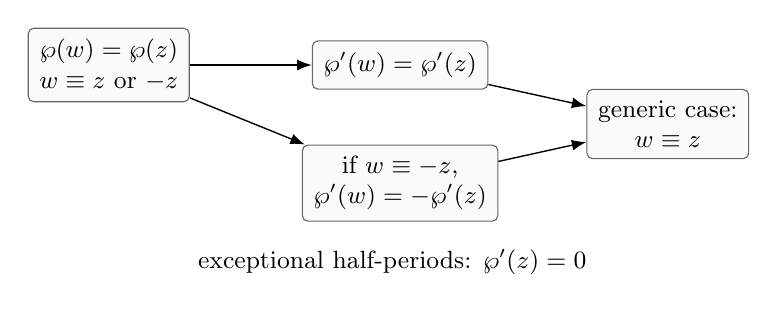
\begin{tikzpicture}[>=Latex, every node/.style={font=\small}]
  \node[smallvisual] (samex) at (0,0.75)
    {$\wp(w)=\wp(z)$\\ \(w\equiv z\) or \(-z\)};
  \node[smallvisual] (samey) at (3.7,0.75)
    {$\wp'(w)=\wp'(z)$};
  \node[smallvisual] (odd) at (3.7,-0.75)
    {if \(w\equiv -z\),\\ \(\wp'(w)=-\wp'(z)\)};
  \node[smallvisual] (concl) at (7.1,0)
    {generic case:\\ \(w\equiv z\)};
  \draw[->, line width=0.5pt] (samex) -- (samey);
  \draw[->, line width=0.5pt] (samey) -- (concl);
  \draw[->, line width=0.5pt] (samex) -- (odd);
  \draw[->, line width=0.5pt] (odd) -- (concl);
  \node[align=center] at (3.6,-1.75)
    {exceptional half-periods: \(\wp'(z)=0\)};
\end{tikzpicture}
\end{center}

\section{Chapter 10}

\textbf{10.1.} In affine coordinates, write \(P=(x_0,y_0)\) and
\(Q=(x_0+h,y(x_0+h))\).  When the tangent is not vertical, the chord slope is
\[
  \frac{y(x_0+h)-y(x_0)}{h}\longrightarrow y'(x_0).
\]
For an implicit equation \(F(x,y)=0\), this derivative is
\[
  y'(x_0)=-\frac{F_x(P)}{F_y(P)}
\]
when \(F_y(P)\ne0\).  The limiting line is the tangent line.  Algebraically, its
intersection with the cubic has a double zero at \(P\), so \(P\) is counted with
intersection multiplicity \(2\).

\begin{center}
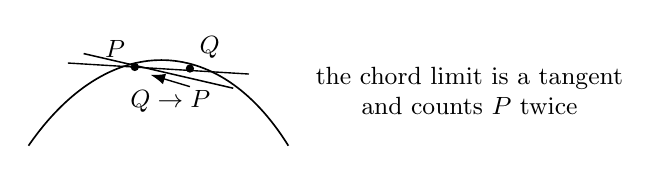
\begin{tikzpicture}[>=Latex, every node/.style={font=\small}]
  \draw[line width=0.6pt] (-1.6,-0.55) .. controls (-0.6,0.9) and (0.8,0.9) .. (1.7,-0.55);
  \fill[black] (-0.25,0.45) circle (1.5pt) node[above left] {$P$};
  \fill[black] (0.45,0.43) circle (1.5pt) node[above right] {$Q$};
  \draw[line width=0.5pt] (-1.1,0.5) -- (1.2,0.36);
  \draw[->, line width=0.5pt] (0.45,0.2) -- (-0.05,0.35) node[midway, below] {$Q\to P$};
  \draw[line width=0.55pt] (-0.9,0.62) -- (1.0,0.18);
  \node[align=center] at (4.0,0.15)
    {the chord limit is a tangent\\and counts \(P\) twice};
\end{tikzpicture}
\end{center}

\textbf{10.2.} Substitute \(y=mx+b\) into
\[
  y^2=4x^3-g_2x-g_3.
\]
The resulting cubic in \(x\) has roots \(x_P,x_Q,x_R\), counted with
multiplicity in the tangent case.  The coefficient of \(x^2\) gives
\[
  x_P+x_Q+x_R=\frac{m^2}{4}.
\]
The chord-tangent sum is the reflection of \(R\), so its \(x\)-coordinate is
\[
  x_{P\boxplus Q}=x_R=\frac{m^2}{4}-x_P-x_Q.
\]

\begin{center}
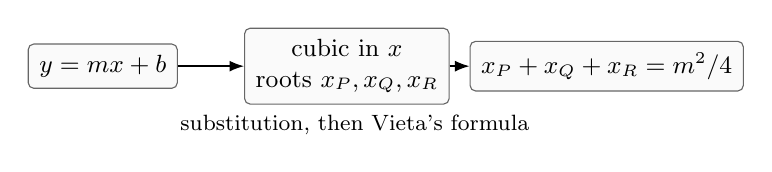
\begin{tikzpicture}[>=Latex, every node/.style={font=\small}]
  \node[smallvisual] (line) at (0,0) {$y=mx+b$};
  \node[smallvisual] (cubic) at (3.1,0)
    {cubic in \(x\)\\roots \(x_P,x_Q,x_R\)};
  \node[smallvisual] (vieta) at (6.4,0)
    {$x_P+x_Q+x_R=m^2/4$};
  \draw[->, line width=0.5pt] (line) -- (cubic);
  \draw[->, line width=0.5pt] (cubic) -- (vieta);
  \node[font=\footnotesize] at (3.2,-0.75) {substitution, then Vieta's formula};
\end{tikzpicture}
\end{center}

\textbf{10.3.} If \(P=(x,y)\), the vertical line \(X=xZ\) gives the affine
intersections \((x,y)\) and \((x,-y)\), since the equation contains \(y^2\).
In projective coordinates the same vertical line also meets the cubic at
\(O=[0:1:0]\).  Thus a vertical line meets \(P\), \(\ominus P\), and \(O\), and
the third intersection construction gives
\[
  P\boxplus(\ominus P)=O.
\]

\begin{center}
\begin{tikzpicture}[>=Latex, every node/.style={font=\small}]
  \begin{scope}[scale=0.55]
    \drawprecisecurve
    \draw[dashed, line width=0.5pt] (0.45,-2.2) -- (0.45,2.2);
    \fill[black] (0.45,1.35) circle (1.7pt) node[above right] {$P$};
    \fill[black] (0.45,-1.35) circle (1.7pt) node[below right] {$\ominus P$};
    \node at (0,-3.2) {$O$};
  \end{scope}
  \node[align=center] at (4.2,0)
    {a vertical line gives the inverse relation\\\(P\boxplus(\ominus P)=O\)};
\end{tikzpicture}
\end{center}

\textbf{10.4.} Let \(f=\ell/h=\ell/Z\) on \(E\).  The zeros of \(f\) are the
zeros of \(\ell|_E\), namely the three intersections of the line \(\ell=0\)
with the cubic:
\[
  [P]+[Q]+[R],
\]
counted with multiplicity.  The poles of \(f\) are the zeros of \(Z|_E\).  On
the Weierstrass cubic,
\[
  Z=0 \quad\Longrightarrow\quad 0=4X^3,
\]
so the line at infinity meets \(E\) only at \(O=[0:1:0]\), with total
intersection multiplicity \(3\).  Hence the pole divisor is \(3[O]\), and
\[
  \divisor(\ell/Z)=[P]+[Q]+[R]-3[O].
\]
Its degree is \(1+1+1-3=0\).

\begin{center}
\begin{tikzpicture}[>=Latex, every node/.style={font=\small}]
  \node[smallvisual] (line) at (0,0.75)
    {\(\ell|_E=0\)\\zeros \(P,Q,R\)};
  \node[smallvisual] (div) at (3.15,0.75)
    {\(Z|_E=0\)\\pole \(3[O]\)};
  \node[smallvisual] (deg) at (3.15,-0.65)
    {\(\divisor(\ell/Z)\)\\ \([P]+[Q]+[R]-3[O]\)};
  \draw[->, line width=0.5pt] (line) -- (div);
  \draw[->, line width=0.5pt] (div) -- node[right] {subtract} (deg);
\end{tikzpicture}
\end{center}

\textbf{10.5.} Since \([P]+[Q]+[R]-3[O]\) is principal, Abel's theorem says its
Abel sum is the identity.  Choose torus preimages \(p,q,r,0\) of \(P,Q,R,O\).
The Abel sum is
\[
  p+q+r-3\cdot0\equiv0\pmod{\Lambda}.
\]
In the transported group law this is exactly
\[
  P+Q+R=O.
\]

\begin{center}
\begin{tikzpicture}[>=Latex, every node/.style={font=\small}]
  \begin{scope}[scale=0.62]
    \drawprecisecurve
    \draw[black, line width=0.65pt]
      (\chordlefta,\chordleftb) -- (\chordrighta,\chordrightb);
    \fill[black] (\chordPx,\chordPy) circle (2pt);
    \node[below left] at (\chordPx,\chordPy) {$P$};
    \fill[black] (\chordQx,\chordQy) circle (2pt);
    \node[above right] at (\chordQx,\chordQy) {$Q$};
    \fill[black] (\chordRx,\chordRy) circle (2pt);
    \node[above left] at (\chordRx,\chordRy) {$R$};
    \node at (0,-3.35) {$O=[0:1:0]$};
  \end{scope}
  \node[align=center] at (5.6,0.2)
    {\([P]+[Q]+[R]-3[O]\in\Prin(E)\)\\[4pt]
     Abel sum \(=0\)\\[4pt]
     \(P+Q+R=O\)};
  \draw[->, line width=0.55pt] (2.7,0.2) -- (4.2,0.2);
\end{tikzpicture}
\end{center}

\section{Chapter 11}

\textbf{11.1.} Abel's theorem is used after the line divisor is known to be
principal.  After choosing torus preimages \(u,v,r\) of \(P,Q,R\), the Abel sum
of the divisor is
\[
  u+v+r-3\cdot0\equiv u+v+r\pmod{\Lambda}.
\]
Abel's theorem converts
\[
  [P]+[Q]+[R]-3[O]\in\Prin(E)
\]
into the group equation \(u+v+r=0\) on the torus.

\begin{center}
\begin{tikzpicture}[>=Latex, every node/.style={font=\small}]
  \node[smallvisual] (line) at (0,0)
    {$[P]+[Q]+[R]-3[O]$\\ principal};
  \node[smallvisual] (abel) at (3.4,0) {Abel's theorem};
  \node[smallvisual] (torus) at (6.5,0) {$u+v+r=0$\\on \(\C/\Lambda\)};
  \draw[->, line width=0.5pt] (line) -- (abel);
  \draw[->, line width=0.5pt] (abel) -- (torus);
\end{tikzpicture}
\end{center}

\textbf{11.2.} A direct proof must compute the third intersection of the line
through \(P,Q\), reflect it to get \(P\boxplus Q\), then compute the third
intersection of the line through \(P\boxplus Q,R\).  The other bracketing
requires the analogous line through \(Q,R\) and then the line through
\(P,Q\boxplus R\).  Comparing the final reflected points is a nonlinear
intersection calculation.  On the torus, the corresponding check is the linear
calculation
\[
  (u+v)+w=u+(v+w).
\]
The transported proof avoids the direct intersection comparison by inheriting
associativity from \(\C/\Lambda\).

\begin{center}
\begin{tikzpicture}[>=Latex, every node/.style={font=\small}]
  \node[smallvisual] (direct) at (0,0.65) {direct cubic proof\\many line intersections};
  \node[smallvisual] (transport) at (0,-0.75) {transported proof\\add in \(\C/\Lambda\)};
  \node[smallvisual] (assoc) at (4.0,-0.75) {associativity is inherited};
  \draw[->, line width=0.5pt] (transport) -- (assoc);
  \draw[dashed, line width=0.45pt] (direct) -- node[right] {harder} (transport);
\end{tikzpicture}
\end{center}

\textbf{11.3.} For \(P=(x,y)\), the projective line \(X=xZ\) contains
\[
  P=(x,y,1),\qquad \ominus P=(x,-y,1),\qquad O=[0:1:0].
\]
Indeed, \(O\) satisfies \(X=xZ\) because both sides are \(0\), and the affine
intersections have the same \(x\)-coordinate with \(y\)-coordinates \(y\) and
\(-y\).  Thus the third intersection of the line through \(O\) and \(P\) is
\(\ominus P\).  Reflecting \(\ominus P\) gives \(P\), so
\[
  O\boxplus P=P.
\]
The case \(P=O\) gives \(O\boxplus O=O\) by the tangent construction at the
identity.

\begin{center}
\begin{tikzpicture}[>=Latex, every node/.style={font=\small}]
  \node[smallvisual] (line) at (0,0)
    {projective line\\\(X=xZ\)};
  \node[smallvisual] (third) at (3.2,0)
    {points\\\(P,\ominus P,O\)};
  \node[smallvisual] (reflect) at (6.15,0)
    {reflect\\\(O\boxplus P=P\)};
  \draw[->, line width=0.5pt] (line) -- (third);
  \draw[->, line width=0.5pt] (third) -- (reflect);
\end{tikzpicture}
\end{center}

\textbf{11.4.} Let \(R=\Phi(r)\) be the third intersection of the line through
\(P=\Phi(u)\) and \(Q=\Phi(v)\).  The line divisor is principal:
\[
  [P]+[Q]+[R]-3[O].
\]
Abel's theorem gives \(u+v+r=0\) in \(\C/\Lambda\), hence
\[
  r=-(u+v).
\]
Reflecting \(R=\Phi(r)\) gives
\[
  \ominus R=\Phi(-r)=\Phi(u+v).
\]
Thus the chord-tangent construction gives the transported torus sum.

\begin{center}
\begin{tikzpicture}[>=Latex, every node/.style={font=\small}]
  \node[smallvisual] (third) at (0,0.8) {$R=\Phi(r)$\\third intersection};
  \node[smallvisual] (abel) at (3.2,0.8) {$u+v+r=0$};
  \node[smallvisual] (neg) at (6.0,0.8) {$r=-(u+v)$};
  \node[smallvisual] (ref) at (3.2,-0.75) {$\ominus R=\Phi(-r)=\Phi(u+v)$};
  \draw[->, line width=0.5pt] (third) -- (abel);
  \draw[->, line width=0.5pt] (abel) -- (neg);
  \draw[->, line width=0.5pt] (neg) -- (ref);
\end{tikzpicture}
\end{center}

\textbf{11.5.} The reflection enters after the third intersection is identified
as \(R=\Phi(r)\) with \(r=-(u+v)\).  Reflection on the cubic corresponds to
\(z\mapsto -z\) on the torus because
\[
  \Phi(-z)=\ominus\Phi(z).
\]
Therefore the reflected point is \(\Phi(-r)=\Phi(u+v)\).

\begin{center}
\begin{tikzpicture}[>=Latex, every node/.style={font=\small}]
  \node[visualnode] (uv) at (0,1.1) {$u,v\in\C/\Lambda$};
  \node[visualnode] (sum) at (4.2,1.1) {$u+v\in\C/\Lambda$};
  \node[visualnode] (PQ) at (0,-0.8) {$P=\Phi(u),\ Q=\Phi(v)$};
  \node[visualnode] (box) at (4.2,-0.8) {$P\boxplus Q$};
  \draw[->, line width=0.55pt] (uv) -- node[above] {add on torus} (sum);
  \draw[->, line width=0.55pt] (uv) -- node[left] {\(\Phi\)} (PQ);
  \draw[->, line width=0.55pt] (sum) -- node[right] {\(\Phi\)} (box);
  \draw[->, line width=0.55pt] (PQ) -- node[below] {chord--tangent} (box);
  \node[align=center] at (2.1,-1.75)
    {The square commutes: \(P\boxplus Q=\Phi(u+v)\).};
\end{tikzpicture}
\end{center}

\section{Chapter 12}

\textbf{12.1.} Under \(g_2\mapsto a^{-4}g_2\) and
\(g_3\mapsto a^{-6}g_3\), one has
\[
  g_2^3\mapsto a^{-12}g_2^3,\qquad
  g_3^2\mapsto a^{-12}g_3^2.
\]
Therefore
\[
  \Delta=g_2^3-27g_3^2\mapsto a^{-12}\Delta.
\]
The common factor \(a^{-12}\) cancels in
\[
  j=1728\frac{g_2^3}{g_2^3-27g_3^2}.
\]

\begin{center}
\begin{tikzpicture}[>=Latex, every node/.style={font=\small}]
  \node[smallvisual] (g2) at (0,0.55) {$g_2^3\mapsto a^{-12}g_2^3$};
  \node[smallvisual] (g3) at (0,-0.55) {$g_3^2\mapsto a^{-12}g_3^2$};
  \node[smallvisual] (j) at (4.4,0) {common factor cancels\\\(j\) is unchanged};
  \draw[->, line width=0.5pt] (g2) -- (j);
  \draw[->, line width=0.5pt] (g3) -- (j);
\end{tikzpicture}
\end{center}

\textbf{12.2.} In genus one, \(H^1(E,\OO_E)\cong\C\) as a complex vector space,
and \(H^1(E,\Z)\cong\Z^2\).  Under the natural map into \(H^1(E,\OO_E)\), the
integral classes give a rank-two lattice \(\Lambda\subset\C\), generated by two
periods.  Therefore
\[
  H^1(E,\OO_E)/H^1(E,\Z)\cong\C/\Lambda.
\]

\begin{center}
\begin{tikzpicture}[>=Latex, every node/.style={font=\small}]
  \node[smallvisual] (vector) at (0,0.6) {$H^1(E,\OO_E)\cong\C$};
  \node[smallvisual] (lattice) at (0,-0.7) {$H^1(E,\Z)\leadsto\Lambda$};
  \node[smallvisual] (quot) at (4.0,0) {$H^1(E,\OO_E)/H^1(E,\Z)\cong\C/\Lambda$};
  \draw[->, line width=0.5pt] (vector) -- (quot);
  \draw[->, line width=0.5pt] (lattice) -- (quot);
\end{tikzpicture}
\end{center}

\textbf{12.3.} For \(\Lambda=\Z+i\Z\), multiplication by \(i\) sends
\[
  1\mapsto i,\qquad i\mapsto -1,
\]
so it preserves the lattice and has order \(4\).  For
\(\Lambda=\Z+\tau\Z\), \(\tau=e^{2\pi i/3}\), multiplication by \(\tau\) sends
\[
  1\mapsto \tau,\qquad \tau\mapsto \tau^2=-1-\tau,
\]
so it preserves the lattice and has order \(3\).  Together with multiplication
by \(-1\), the hexagonal lattice has rotations of order \(6\).  These rotations
suggest extra automorphisms.

\begin{center}
\begin{tikzpicture}[>=Latex, every node/.style={font=\small}]
  \node[smallvisual] (square) at (0,0)
    {$\tau=i$\\square lattice\\order \(4\) rotation};
  \node[smallvisual] (hex) at (4.0,0)
    {$\tau=e^{2\pi i/3}$\\hexagonal lattice\\order \(6\) rotation};
  \draw[->, line width=0.5pt] (square) -- node[above] {extra symmetry} (hex);
\end{tikzpicture}
\end{center}

\textbf{12.4.} The quotient re-expresses the identification
\[
  \Pic^0(E)\cong\C/\Lambda.
\]
It explains the Jacobian as a complex torus.  It does not by itself prove the
chord-tangent formula.  Two further calculations are needed: first, the line
section calculation
\[
  \divisor(L|_E)=[P]+[Q]+[R]-3[O],
\]
and second, the Abel-sum calculation \(u+v+r\equiv0\pmod{\Lambda}\), which turns
that divisor into the group equation.

\begin{center}
\begin{tikzpicture}[>=Latex, every node/.style={font=\small}]
  \node[smallvisual] (coh) at (0,0.65)
    {cohomology quotient\\\(\Pic^0(E)\cong\C/\Lambda\)};
  \node[smallvisual] (line) at (4.2,0.65)
    {line divisor\\on the cubic};
  \node[smallvisual] (abel) at (4.2,-0.85)
    {Abel's theorem};
  \node[smallvisual] (law) at (0,-0.85)
    {chord--tangent law};
  \draw[->, line width=0.5pt] (coh) -- (line);
  \draw[->, line width=0.5pt] (line) -- (abel);
  \draw[->, line width=0.5pt] (abel) -- (law);
\end{tikzpicture}
\end{center}

\section{Chapter 13}

\textbf{13.1.} Over \(\F_5\), compute \(x^3+2x+1\):
\[
  1,4,3,4,3
\]
for \(x=0,1,2,3,4\).  The quadratic residues modulo \(5\) are \(0,1,4\).
Thus \(x=0\) gives two points, \(x=1\) gives two points, \(x=2\) gives none,
\(x=3\) gives two points, and \(x=4\) gives none.  Adding the point at infinity
gives \(\#E(\F_5)=7\).

\begin{center}
\begin{tikzpicture}[>=Latex, every node/.style={font=\small}]
  \foreach \x/\val/\pts in {0/1/2,1/4/2,2/3/0,3/4/2,4/3/0}{
    \node[smallvisual, minimum width=1.15cm] at (1.25*\x,0)
      {$x=\x$\\ \(f(x)=\val\)\\ \(\pts\) pts};
  }
  \node[smallvisual] at (6.9,0) {$+O$\\ total \(7\)};
  \draw[->, line width=0.5pt] (5.35,0) -- (6.1,0);
\end{tikzpicture}
\end{center}

\textbf{13.2.} The chord-tangent formulas use addition, subtraction,
multiplication, and division by a nonzero denominator.  For example, the slope is
\[
  m=\frac{y_Q-y_P}{x_Q-x_P}
\]
for a nonvertical chord, and the tangent slope is obtained by a similar quotient
involving the derivative.  Therefore the formulas make sense over any field
where the curve is smooth.  The exceptional denominator cases are vertical
lines, the point at infinity, coincident points requiring the tangent formula,
and tangent denominators equal to zero.

\begin{center}
\begin{tikzpicture}[>=Latex, every node/.style={font=\small}]
  \node[smallvisual] (smooth) at (0,0)
    {smooth cubic over \(k\)};
  \node[smallvisual] (ops) at (3.0,0)
    {field operations\\in \(k\)};
  \node[smallvisual] (law) at (6.0,0)
    {chord--tangent\\group law};
  \draw[->, line width=0.5pt] (smooth) -- (ops);
  \draw[->, line width=0.5pt] (ops) -- (law);
\end{tikzpicture}
\end{center}

\textbf{13.3.} The Hasse bound says that \(\#E(\F_p)\) lies within
\(2\sqrt p\) of \(p+1\).  Geometrically, the number of finite-field points is
close to the projective-line count \(p+1\), with a square-root-size error.

\begin{center}
\begin{tikzpicture}[>=Latex, every node/.style={font=\small}]
  \draw[->, black!55, line width=0.45pt] (-3.1,0) -- (3.3,0);
  \draw[line width=0.6pt] (-2.0,0.12) -- (2.0,0.12);
  \fill[black] (0,0.12) circle (1.5pt) node[above] {$p+1$};
  \node[below] at (-2.0,0) {$p+1-2\sqrt p$};
  \node[below] at (2.0,0) {$p+1+2\sqrt p$};
  \node[align=center] at (0,-1.05)
    {\(\#E(\F_p)\) lies in this interval};
\end{tikzpicture}
\end{center}

\textbf{13.4.} The requested separation is:
\[
\begin{array}{c|c}
\text{algebraic over a general field} & \text{analytic over }\C\\ \hline
\text{smooth cubic equation} & \text{lattice }\Lambda\subset\C\\
O=[0:1:0] & \C/\Lambda\\
\text{divisors and divisor classes} & \wp,\wp'\\
\text{rational chord--tangent formulas} & \text{period integrals}\\
E(k) \text{ for a field } k & \text{complex Lie group structure}
\end{array}
\]
The analytic uniformization
\[
  E(\C)\cong\C/\Lambda
\]
uses complex analysis, lattices in \(\C\), and meromorphic functions such as
\(\wp\); that part is special to the complex setting.

\begin{center}
\begin{tikzpicture}[>=Latex, every node/.style={font=\small}]
  \node[smallvisual] (alg) at (0,0.65)
    {algebraic cubic\\works over many fields};
  \node[smallvisual] (ct) at (4.0,0.65)
    {chord--tangent formulas};
  \node[smallvisual] (complex) at (0,-0.85)
    {analytic uniformization\\needs \(\C\), \(\Lambda\), \(\wp\)};
  \node[smallvisual] (torus) at (4.0,-0.85)
    {\(E(\C)\cong\C/\Lambda\)};
  \draw[->, line width=0.5pt] (alg) -- (ct);
  \draw[->, line width=0.5pt] (complex) -- (torus);
\end{tikzpicture}
\end{center}

\section{Chapter 14}

\textbf{14.1.} A line through \(P,Q,R\) makes
\[
  [P]+[Q]+[R]-3[O]
\]
principal.  Abel's theorem gives the group equation
\[
  P+Q+R=O.
\]
Solving for the group sum gives \(P+Q=-R=\ominus R\).  The chord--tangent rule
therefore defines \(P\boxplus Q=\ominus R\); the reflection step is forced by
the group equation.

\begin{center}
\begin{tikzpicture}[>=Latex, every node/.style={font=\small}]
  \node[smallvisual] (line) at (0,0.75)
    {line through \(P,Q,R\)};
  \node[smallvisual] (abel) at (3.15,0.75)
    {$P+Q+R=O$};
  \node[smallvisual] (reflect) at (3.15,-0.7)
    {\(P\boxplus Q=-R\)\\reflection is forced};
  \draw[->, line width=0.5pt] (line) -- (abel);
  \draw[->, line width=0.5pt] (abel) -- node[right] {reflect} (reflect);
  \node[font=\footnotesize] at (1.55,0.25) {Abel's theorem};
\end{tikzpicture}
\end{center}

\textbf{14.2.} One possible table is:
\[
\begin{array}{c|c|c}
\text{analytic} & \text{divisor-theoretic} & \text{algebraic}\\ \hline
\C/\Lambda,\wp & \Pic^0(E),\text{ divisors} & E(\C),\text{ lines}\\
\Phi=[\wp:\wp':1] & \text{Abel--Jacobi} & P\mapsto[P]-[O]
\end{array}
\]
The first map sends the torus to the cubic, and the second sends a cubic point
to its degree-zero divisor class.

\begin{center}
\begin{tikzpicture}[>=Latex, every node/.style={font=\small}]
  \node[smallvisual] (T) at (0,1.2) {analytic\\\(\C/\Lambda,\wp\)};
  \node[smallvisual] (J) at (-2.6,-0.8) {geometric\\\(\Pic^0(E)\)};
  \node[smallvisual] (E) at (2.6,-0.8) {algebraic\\\(E(\C)\), lines};
  \draw[->, line width=0.5pt] (T) -- node[above right] {\(\Phi\)} (E);
  \draw[->, line width=0.5pt] (E) -- node[below] {$P\mapsto[P]-[O]$} (J);
  \draw[->, line width=0.5pt] (J) -- node[above left] {Abel--Jacobi} (T);
\end{tikzpicture}
\end{center}

\textbf{14.3.} A compact chapter-to-method table is:
\[
\begin{array}{c|c|c}
\text{chapters} & \text{viewpoint} & \text{calculation type}\\ \hline
1\text{--}2 & \text{complex-analysis background} & \text{residues, integrals, genus}\\
3\text{--}5 & \text{analytic torus} & \text{lattice algebra, pole orders}\\
6\text{--}8 & \text{divisors and Jacobian} & \text{divisor coefficients, Abel sums}\\
9\text{--}11 & \text{plane cubic} & \text{Vieta and line intersections}\\
12 & \text{cohomology and moduli} & \text{quotients and scaling weights}\\
13 & \text{arithmetic} & \text{finite-field point counts}
\end{array}
\]

\begin{center}
\begin{tikzpicture}[>=Latex, every node/.style={font=\small}]
  \node[smallvisual] (a) at (0,0) {Ch. 3--5\\analytic};
  \node[smallvisual] (b) at (2.4,0) {Ch. 6--8\\divisors};
  \node[smallvisual] (c) at (4.8,0) {Ch. 9--11\\cubic};
  \node[smallvisual] (d) at (7.2,0) {Ch. 12--13\\extensions};
  \draw[->, line width=0.5pt] (a) -- (b);
  \draw[->, line width=0.5pt] (b) -- (c);
  \draw[->, line width=0.5pt] (c) -- (d);
\end{tikzpicture}
\end{center}

\textbf{14.4.} A compact map-check table is:

\begin{center}
\scriptsize
\setlength{\tabcolsep}{2pt}
\begin{tabular}{|L{1.15cm}|L{2.05cm}|L{1.35cm}|L{1.35cm}|L{2.35cm}|L{2.25cm}|L{2.45cm}|}
\hline
map & formula & source & target & group-law compatibility &
holomorphicity input & inverse or bijectivity input\\
\hline
\(\Phi\) &
\(z\mapsto[\wp(z):\wp'(z):1]\) &
\(\C/\Lambda\) &
\(E(\C)\) &
direct transport calculation:
\(\Phi(u+v)=\Phi(u)\boxplus\Phi(v)\) after Ex. 11.4 &
calculation with meromorphic coordinates and the projective limit at \(O\);
global extension is theorem input &
Weierstrass embedding theorem; Ex. 9.6 gives only the generic injectivity
calculation\\
\hline
\(AJ\) &
\(P\mapsto[P]-[O]\) &
\(E(\C)\) &
\(\Pic^0(E)\) &
Abel-sum calculation in Ex. 14.5 plus Abel's theorem &
accepted Jacobian/Abel-Jacobi theorem input &
Abel's theorem and genus-one representative statement\\
\hline
\end{tabular}
\end{center}

Thus the final isomorphism as complex Lie groups uses direct calculations for
the formulas, Abel sums, reflection step, and transported addition, and uses
named theorems for the global biholomorphic and Jacobian-identification inputs.

\begin{center}
\begin{tikzpicture}[>=Latex, every node/.style={font=\small}]
  \node[smallvisual] (T) at (0,0) {$\C/\Lambda$};
  \node[smallvisual] (E) at (3.0,0) {$E(\C)$};
  \node[smallvisual] (P) at (6.0,0) {$\Pic^0(E)$};
  \draw[->, line width=0.5pt] (T) -- node[above] {\(\Phi\)} (E);
  \draw[->, line width=0.5pt] (E) -- node[above] {$P\mapsto[P]-[O]$} (P);
  \node[align=center] at (3.0,-0.95)
    {both maps preserve complex structure and addition};
\end{tikzpicture}
\end{center}

\textbf{14.5.} A point \(z\in\C/\Lambda\) is written on the cubic as
\[
  \Phi(z)=[\wp(z):\wp'(z):1],
\]
and in the Jacobian as
\[
  [\Phi(z)]-[O].
\]
Adding \(z_1,z_2\) on the torus gives \(z_1+z_2\).  On the cubic this is
\[
  \Phi(z_1)\oplus\Phi(z_2)=\Phi(z_1+z_2),
\]
which equals the chord-tangent construction.  In the Jacobian it is addition of
divisor classes:
\[
  ([\Phi(z_1)]-[O])+([\Phi(z_2)]-[O]).
\]
If \(S=\Phi(z_1+z_2)\), then Abel's theorem gives
\[
  [\Phi(z_1)]+[\Phi(z_2)]-[S]-[O]\in\Prin(E)
\]
because its Abel sum is
\[
  z_1+z_2-(z_1+z_2)-0\equiv0\pmod{\Lambda}.
\]
Therefore the class of this divisor is zero in \(\Pic^0(E)\), so
\[
  [\Phi(z_1)]+[\Phi(z_2)]-2[O]=[S]-[O].
\]
Equivalently,
\[
  ([P_1]-[O])+([P_2]-[O])=[S]-[O]
\]
for \(P_i=\Phi(z_i)\) and \(S=\Phi(z_1+z_2)\).

\begin{center}
\begin{tikzpicture}[>=Latex, every node/.style={font=\small}]
  \node[visualnode] (z) at (0,0.95) {$z\in\C/\Lambda$};
  \node[visualnode] (P) at (4.6,0.95) {$\Phi(z)\in E(\C)$};
  \node[visualnode] (D) at (2.3,-0.85) {$[\Phi(z)]-[O]\in\Pic^0(E)$};
  \draw[->, line width=0.55pt] (z) -- node[above] {\(\Phi=[\wp:\wp':1]\)} (P);
  \draw[->, line width=0.55pt] (P) -- node[right] {\(\;P\mapsto[P]-[O]\)} (D);
  \draw[->, line width=0.55pt] (D) -- node[left] {Abel--Jacobi} (z);
  \node[align=center] at (2.3,-1.8)
    {one group element, three notations};
\end{tikzpicture}
\end{center}


\backmatter

\begin{thebibliography}{9}
\bibitem{ahlfors}
L. V. Ahlfors, \emph{Complex Analysis}, 3rd ed., McGraw--Hill, 1979.

\bibitem{miranda}
R. Miranda, \emph{Algebraic Curves and Riemann Surfaces}, American Mathematical
Society, 1995.

\bibitem{silverman}
J. H. Silverman, \emph{The Arithmetic of Elliptic Curves}, 2nd ed., Springer,
2009.

\bibitem{silverman-tate}
J. H. Silverman and J. Tate, \emph{Rational Points on Elliptic Curves}, 2nd ed.,
Springer, 2015.

\bibitem{forster}
O. Forster, \emph{Lectures on Riemann Surfaces}, Springer, 1981.
\end{thebibliography}

\end{document}
